% Chapter Template

\chapter{Efficacy Transition Pathways} % Main chapter title

\label{etp} % For referencing this chapter elsewhere, use \ref{etp}

%----------------------------------------------------------------------------------------
%	SECTION 1
%----------------------------------------------------------------------------------------

\section{Introduction}
\label{etp:Introduction}

Phase \RN{2} trials build upon the work of early Phase \RN{1} trials where preliminary information is obtained regarding the safety profile and dose schedule of a treatment. The key output from a Phase \RN{1} trial is the MTD (Maximum Tolerated Dose), TD\%\% (target dose at some pre-specified level), RP2D (Recommended Phase \RN{2} Dose) or OBD (optimal biological dose) i.e. some dose-level that can be taken forward for future testing. In Phase \RN{2} trials the focus shifts away from toxicity and looks more towards efficacy of these new treatments at the dose-levels previously defined \cite{berryBayesianAdaptiveMethods2010}. The purpose of phase \RN{2} trials is to usually see if a new treatment or intervention works and establish if there is a efficacy signal. More specifically they aim to determine if there is a sufficient level of efficacy to warrant further research in for example a Phase \RN{3} setting \cite{juliousIntroductionStatisticsEarly2010}. In addition to assessing efficacy there is also opportunity to further explore the toxicity profile of the treatment as in comparison to Phase \RN{1} trials Phase \RN{2} trials are typically conducted using a larger sample size.  

Phase \RN{2} trials can be categorised further, dependent on the primary aims of the trial. Single-arm trials can be classified as Phase \RN{2} A trials, here a sample of patients would be given the experimental treatment and efficacy would be assessed. There are also multi-arm trials which may randomise patients to multiple experimental treatments or between an experimental treatment and standard of care. Efficacy would then be compared across the different arms. These types of trials are commonly referred to as Phase \RN{2} B trials. 

Generally speaking Phase \RN{2} trials should be efficient and quick such that we can progress to Phase \RN{3} as quickly as possible or drop any ineffective treatments. The output from a Phase \RN{2} trial should be either a 'GO' or 'No GO' decision i.e should we or should we not proceed to later phase testing based on the data observed in this trial. One of the more important aspects of these trials is that we don't want to make any incorrect decisions and if there is an effective treatment that is being investigated we want to make sure that it is taken forward into Phase \RN{3}.

An example of a Phase II single arm trial design is depicted in Figure \ref{fig_etp:phase2_singlearm_example}. For single-arm Phase \RN{2} trials eligible patients come into the trial and all of them will be allocated to the new treatment. Once they have completed their treatment period we would then assess the effectiveness of that treatment using some measure of success. Looking at the outcome of success in each patient the success rate or proportion of success can then be determined. In the single arm setting, this success rate is then compared to some sort of benchmark, which is determined from either historical data or clinical input.


\begin{figure}[h!]
	\centering
	\caption{Example of a Phase 2 single arm trial design.}
	\label{fig_etp:phase2_singlearm_example}
	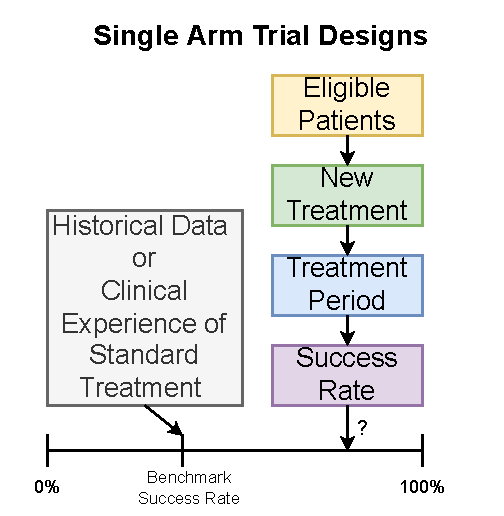
\includegraphics[width=0.75\textwidth]{ETP-Phase2SingleArmExample}
\end{figure}

The primary outcome measure for a trial like this should be some short-term binary outcome either success or failure. The outcome measure selected should be chosen such that you expect the treatment to have an effect on that. Typically these are surrogates for longer-term efficacy measures. So, if we see a success in the Phase II trial we would hope there would also be some long-term benefits for patients as well. In the oncology setting Phase III trials typically will look at outcomes such as survival times but in the previous Phase II trials response or change in tumour size may have been used as outcomes.

There are many classical frequentist approaches which can be applied to Phase \RN{2} trials such as the Flemming A'Hern, Simons two-stage or Bryant and Day designs. However, there exist complex and innovative designs that are adaptive in nature and allow for more frequent interim analyses so decisions can be made faster. 

One approach is Bayesian and utilises a Beta-Binomial conjugate analysis to estimate a  response rate for a binary outcome. Posterior probabilities can be used to inform decision making and predictive probabilities can be used during interim analyses in a similar manner. This is typically done using pre-specified decision rules.

Whilst mathematically simple to implement a design such as this has similar drawbacks to dose-finding methodologies that have been previously discussed. Due to its flexibility there may be some issues with parametrising the design, in this case would mean selecting the correct decision rules. A Bayesian approach may be less familiar than traditional frequentist approaches that are more commonly used. It may also be hard to understand why certain decisions are being made during interim and final analyses.  

One potential solution to these problems was devised by Lucinda Billingham who developed Efficacy Transition Pathways (ETPs) a novel visualisation tool to aid the design and interpretation of these types of trial designs. ETPs extend on the idea of dose transition pathways, which solves for many of the same issues in dose-finding trials. 

In this chapter we will explore the components that go into constructing an ETP for a Beta-Binomial conjugate analysis. We will detail how ETPs can be used in a trial setting with an illustrative example. Finally, we also provide details on a web application that can be used to produce ETPs and acts as an educational tool to explain what they are. 

%----------------------------------------------------------------------------------------
%	SECTION 2
%----------------------------------------------------------------------------------------

\section{Beta-Binomial Conjugate Analyses}
\label{etp:BBConjugateAnalysis}

Bayesian methods are an alternative way of thinking about evidence, data and statistics compared to the traditional frequentist approach. The Bayesian approach could be considered more intuitive and has some advantages that make it useful for analysing clinical trials. 

The fundamentals of Bayesian statistics are well defined in the literature as well as its application to clinical trials and health research. Bland and Altman \cite{blandBayesiansFrequentists1998} discuss the differences between a Bayesian or a frequentist approach. Spiegelhalter et al. \cite{spiegelhalterIntroductionBayesianMethods1999} detail the underlying philosophy behind Bayesian methods along with its application in health technology assessment. General Bayesian methods are described in more detail in books by Lee \cite{leeBayesianStatisticsIntroduction2012} and Bernado and Smith \cite{bernardoBayesianTheory2009}. It should be noted, these are just a few examples from the literature.    

The Bayesian paradigm doesn’t regard parameters, things we don’t know like a treatment effect ($\theta$), as fixed. These are instead thought of to be uncertain. Bayesian statistics uses probability to express this uncertainty. Since $\theta$ is unknown, it has a probability distribution. 

Bayesian analysis takes into account prior information on $\theta$ which also has the form of a probability distribution. This is combined with the likelihood of the data, Y given $\theta$, to produce a posterior probability distribution of $\theta$ given Y. So, data is collected to find out about the parameter. This data can be regarded as known and fixed and is used to estimate the unknown parameter. In Bayesian statistics, we estimate the probability of the parameter given the data.

Once a posterior distribution is established inferences can then be made about $\theta$. However, this may require numerical integration of the posterior distribution which may be difficult or impossible to evaluate analytically. An option around this is to use conjugate priors. If the posterior distribution and the prior distribution are from the same probability distribution family these can be referred to as conjugate distributions and the prior as a conjugate prior. Conjugate priors are algebraically easier to deal with and allow for easier interpretation of the posterior distribution. 

One example of this is what is commonly referred to as the Beta-Binomial conjugate. This is where the prior and posterior distributions take the form of a Beta distribution and the likelihood or data is Binomial. 

Binomial data has two possible outcomes. For example, a coin toss has two outcomes either its head or its tails. In the context of a Phase II single arm trial, this could be either a success/failure to some new treatment or response/no response. When this is combined with a Beta prior distribution we get a posterior Beta distribution. From this, we can then make probability statements about the treatment effect.

Following the explanation by Lee \cite{leeBayesianStatisticsIntroduction2012} of a Beta conjugate prior for a binomial distribution. Consider a parameter of interest $\theta$ that represents some treatment effect. More specifically, for binomial data in a single arm Phase \RN{2} clinical trial, lets say the parameter $\theta$ is the probability of response in a number of patients following a some new treatment. Each patient can experience either a response or no response, with the same probability of response and each patient being independent from each other. For a fixed sample size with $n$ patients and number of responses ($y$) we have: 

\begin{equation}
	Y \sim \text{Binomial}(n, \theta)
\end{equation}

So, $y$ is from a binomial distribution which produces the following likelihood: 

\begin{equation}
	L(\theta) = P(y|\theta) = {n \choose y}\theta^y (1-\theta)^{n-y} \; \; \; \; (y = 0,1,\ldots,n)
\end{equation}

If the prior for $\theta$ is from a Beta distribution such that 

\begin{equation}
	\label{eq_etp:betaprior}
	P(\theta) = \text{Beta}(a,b)
\end{equation}

then the posterior distribution is also from a Beta distribution and can be expressed as 

\begin{equation}
\label{eq_etp:betaposterior}
	P(\theta|y) = \text{Beta}(a+y,b+n-y)
\end{equation}

To avoid confusion with the prior we will let $\alpha = a+y$ and $\beta = b+n-y$ which gives

\begin{equation}
	\label{eq_etp:betaposterior2}
	P(\theta|y) = \text{Beta}(\alpha,\beta)
\end{equation}

Bayesian inference can then be used for estimation and decision making. Features such as the mean and  variance of the treatment effect $\theta$ can be  estimated from the posterior distribution given in equation \ref{eq_etp:betaposterior2}. For the posterior distribution of $\theta \sim Beta(\alpha,\beta)$ the mean, variance and mode are.

\begin{equation}
\label{eq_etp:betamean}
	E[\theta] = \frac{\alpha}{\alpha + \beta} 
\end{equation}

\begin{equation}
\label{eq_etp:betavar}
	Var[\theta] = \frac{\alpha\beta}{(\alpha+\beta)^2 (\alpha+\beta+1)}
\end{equation}

\begin{equation}
	\label{eq_etp:betamode}
	mode[\theta] = \frac{\alpha - 1 }{\alpha + \beta - 2} 
\end{equation}
 
The proofs for these formula are relatively simple and can be found in \cite{sochBookStatisticalProofs2020}. There exists no closed formula for the median however this can still be calculated using the density function of a Beta distribution. If we take $\theta^m$ to be the median then, the median is the value that solves 

\begin{equation}
	P(\theta < Median) = 0.5 = \int_{0}^{\theta^m} \theta^{\alpha-1}(1-\theta)^{\beta-1}d\theta
\end{equation}

Alternatively, there is a closed form approximation to the median presented by Kerman \cite{kermanClosedformApproximationMedian2011} which is as follows 

\begin{equation}
	median[\theta] \approx \frac{\alpha - \frac{1}{3}}{\alpha + \beta - \frac{2}{3}}
\end{equation}

We can also establish credible intervals or make other probability statements in a similar manner. 
Then pre-specified rules based on these direct probabilities from the posterior can be used for decision making purposes. For example, if 

\begin{equation}
	\label{eq_etp:betafinaldecrule}
	P(\theta > c |y) \geq q  \; \; \; \; \text{then GO else No GO}
\end{equation}


where $c$ is some target level of treatment effect and $q$ is some threshold of sufficient evidence. This probability can be calculated from the density function of the Beta distribution from $c$ to $\infty$. 

\begin{equation}
	P(\theta > c | y) = \int_{c}^{\infty}\theta^{\alpha-1}(1-\theta)^{\beta-1}d\theta
\end{equation}

It should be noted that $\int_{0}^{1}\theta^{\alpha-1}(1-\theta)^{\beta-1}d\theta = 1$, so $\theta$ has an upper bound of 1. Appropriate decision criteria, i.e. values for $c$ and $q$, can be determined and evaluated via simulations.

%-----------------------------------
%	SUBSECTION 1
%-----------------------------------

\subsection{Illustrative example to showcase a Beta-Binomial design} 
\label{etp:BBIllEx}
In this section we will detail an example to show how a Beta-Binomial conjugate analysis would work in practice and how its used to make decisions. 

Consider a trial in which we are trying to evaluate the efficacy of some new treatment. This will be done using an outcome measure of response. Patients can either be considered a responder or a non-responder. The treatment effect will be the response rate and will be analysed using a Beta-Binomial conjugate model. 

To conduct the analysis and make a GO or No GO decision a prior and decision criteria needs to be specified. For simplicity a minimally informative Beta(1,1) prior will be used. This represents a 50\% response rate from a group of two patients. The following decision rule will also be used $P(\theta  \geq 30\%) \geq 0.9$, where $\theta$ is the treatment effect (response rate). So, if there is a greater than  90\% chance that the true response rate is at least 30\% this will be considered sufficient evidence to warrant a GO decision. 

Now assume that 30 patients were recruited 16 of which had a response. Using equation \ref{eq_etp:betaposterior} we can establish that the posterior distribution for the treatment effect is $P(\theta) = \text{Beta}(17, 15)$. From this we can then calculate summary estimates, which are presented in Table \ref{tab_etp:bb_sum_est}.

\begin{table}[H]
	\centering
	\caption{Summary estimates of response rate with 30 patients and 16 responses. }
	\label{tab_etp:bb_sum_est}
	\begin{tabular}{cc}
		\hline
		\textbf{Summary Estimate}                   &              \\ \hline
		\multicolumn{1}{c|}{Mean}                   & 0.531        \\
		\multicolumn{1}{c|}{Median}                 & 0.532       \\
		\multicolumn{1}{c|}{Mode}                   & 0.533          \\
		\multicolumn{1}{c|}{Variance}               & 0.008        \\
		\multicolumn{1}{c|}{95\% Credible Interval} & 0.360, 0.698 \\ \hline
	\end{tabular}
\end{table}

From these estimates we can say, based on the data that is observed (16 responses in 30 patients), the response rate is 53\% with a 95\% credible interval (36\%, 70\%). The probability of the response rate being at least 40\% can also be calculated. In this example it is 99.7\%. As this value is greater than the threshold of 90\%  we can say there is sufficient evidence to warrant a GO decision.

This can also be illustrated as shown in Figure \ref{fig_etp:bb_dec_rule1}. The blue shaded region highlights the upper 90\% of the distribution. In this scenario with this decision criteria, as the entire region does not cross the target response rate of 30\% we have a GO decision. We can see that there is a greater than 90\% chance that the response rate is greater than 30\%. 

 \begin{figure}[h!]
 	\centering
 	\caption{Posterior distribution of response rate with decision criteria.}
 	\label{fig_etp:bb_dec_rule1}
 	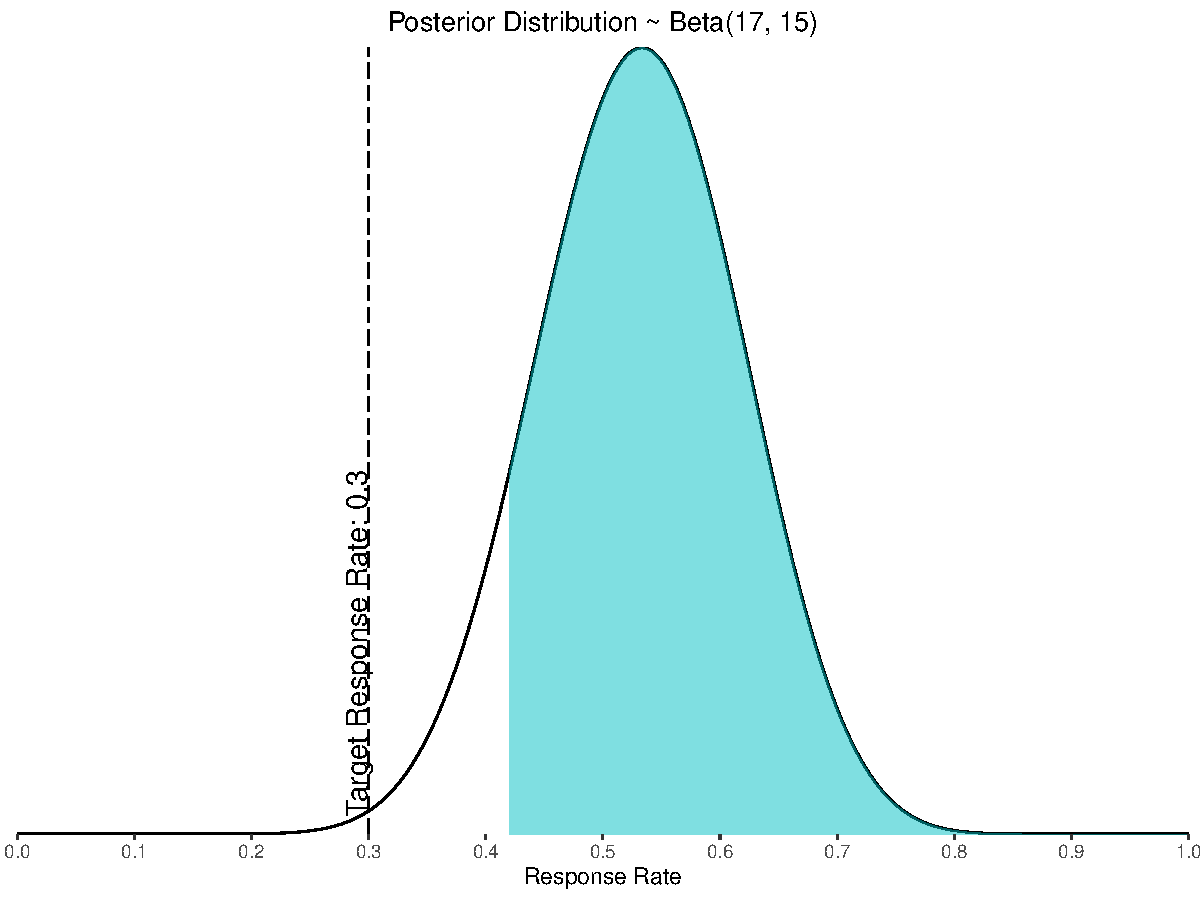
\includegraphics[width=\textwidth]{ETP-BetaBinomialDecRule1}
 \end{figure}

In practice decision rules should be decided before the trial starts. This is typically done via the evaluation of simulations. Multiple scenarios corresponding to different true response rates can be investigated. The probability of making a correct decision can then be calculated. This represents the power of our design. For scenarios with low true response rates (relative to the target response rate) we want the probability of making a No GO decision to be high. Similarly, for scenarios with high true response rates we want the probability of making a GO decision to be high. The decision rule parameters, the target response rate and probability threshold can then be adjusted to ensure the design is making appropriate decisions in these scenarios. 

Simulations can also be used to evaluate the choice of prior as well. A variety of different priors can be used dependent on the trial. A prior like the Beta(1,1) is typically described as minimally informative. This means that if the data observed is reasonably large the likelihood will dominate and have more influence on the posterior. So, if we observe a really strong treatment effect this will be reflected in the posterior. 

A sceptical prior can be used when we are sceptical about the treatment producing large treatment effects. These are typically centred around a low treatment effect whilst still leaving some scope for their to be plausible positive treatment effect. The opposite of this would be a enthusiastic prior. Here the prior would be centered around a high treatment effect whilst allowing some possibility for a negative treatment effect.

Priors can also be evidence based or elicited. Evidence based priors will use results or data from previous trials to inform the choice of prior. These can then be adjusted to account for any potential biases. Elicited priors are decided based on discussions with a group of experts. 

Figure \ref{fig_etp:bb_example_priors} shows the effect that different priors can have on the estimation of the treatment effect. Our example with 16 responses and a minimally informative prior is shown in the first plot. Here we can see the median response rate is 53.2\% and the probability of the response rate being greater than 30\% is greater than 90\% meaning we have a go decision. The minimally informative prior is indicated by the red line and is essentially a uniform distribution. Assuming we still have 16 responses, we can see that when a sceptical Beta(2,8) prior is implemented the posterior distribution changes from Beta(17,15) to Beta(18,22). This shifts the posterior such that the new estimated median response rate is 44.9\%. However even with a sceptical prior we can still see we meet the criteria for a GO decision with a probability of 0.976 that the response rate is greater than 30\%. Then with an enthusiastic prior the posterior shifts in the other direction. So, with the same 16 responses but an enthusiastic prior the estimate of the response rate is 57.6\%. Again, the decision criteria is also met in this instance as well.    

 \begin{figure}[h!]
	\centering
	\caption{Posterior distribution of example under different priors.}
	\label{fig_etp:bb_example_priors}
	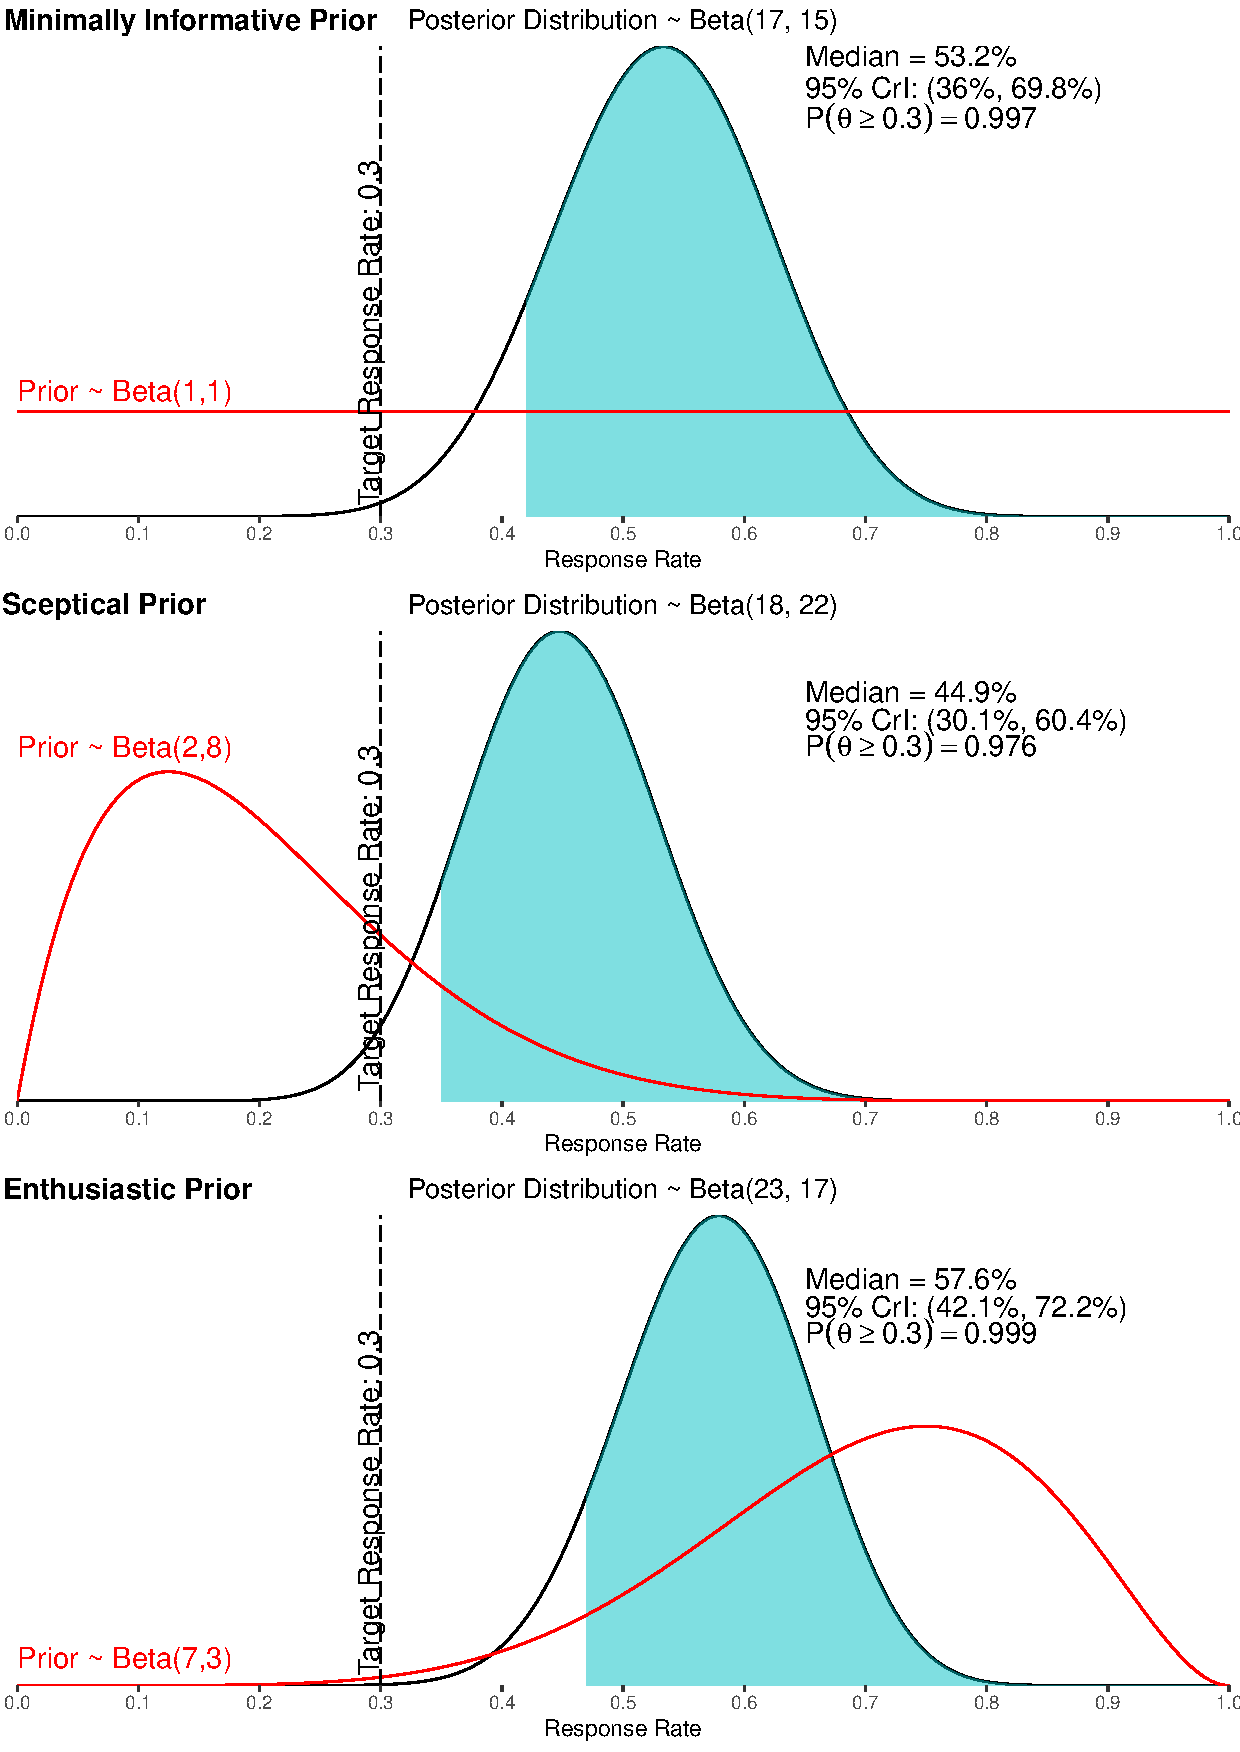
\includegraphics[width=\textwidth]{ETP-BetaBinomialPriors}
\end{figure}

In this example the choice of prior did not impact the decision that would be made. However, if the decision rule was different or the number of responses seen was less this could change. As part of some trials a sensitivity may be conducted to check the results and decisions of a trial with a different prior. As stated before simulation work is used to establish the most appropriate decision criteria and priors can be sourced from available evidence or elicited. The simulations should be conducted with the priors in mind as well as any sensitivity analyses that may be planned.   

Once the decision rule and prior have been specified the minimum number of responses required to make a GO decision could also be calculated. In our example here this number is 13. So, we would need to observe a minimum of 13 responses to make a GO decision out of 30 patients. To make these trial designs more efficient interim analyses can be included. This will allow the trial to look at the data at an earlier time point and potentially make a decision earlier as to whether the trial should continue. In the next section we look at how the predictive probability of success (PPOS) is used to make decisions at interim analyses. 

%-----------------------------------
%	SUBSECTION 3
%-----------------------------------

\subsection{Interim analyses and Predictive Probability of Success}

There are several different methods in which interim analyses can be incorporated into a single-arm Phase \RN{2} clinical trial. One method that can be used in the context of a Beta-Binomial conjugate analysis utilises PPoS. This works by evaluating the data at pre-specified time points or after a certain intervals of patients have been recruited. At these time points we can determine whether or not we have observed enough responses to warrant continuing with the trial based on the overall minimum responses we would need for a final GO decision. More explicitly the PPoS is the probability of the trial being considered a success given the current data observed at the interim analysis. This is calculated by predicting the future number of responses in the patients yet to be recruited based on the data that has already been observed. 

In section \ref{etp:BBConjugateAnalysis} we detailed how a Beta-Binomial conjugate analysis works in practice. Here, we will extend that to show how PPoS and an interim analysis can be incorporated into this trial design following the explanation of Berry et al. \cite{berryBayesianAdaptiveMethods2010}. 

Consider for a fixed sample of size $n$ patients an interim analysis that will be conducted after $n_{int}$ patients, such that $n_{int} < n$. Again, the parameter of interest, treatment effect or response rate will be represented by $\theta$. Let the number of responses $x$ among the $n_{int}$ patients follow a binomial distribution: 

\begin{equation}
	X \sim \text{Binomial}(n_{int},\theta) 
\end{equation}

Let $Z$ be the number of responses in the remaining $m$ patients, where $m = n - n_{int}$. When $Z = i$, where $i = 1, ..., m$, the posterior distribution can be expressed as 

\begin{equation}
	P(\theta|x,Z=i) = \text{Beta}(a+x+z, b+n-x-z)
\end{equation}

Where $a$ and $b$ are parameters from the Beta prior distribution, see equation \ref{eq_etp:betaprior}. 

Suppose we have a decision rule where a GO decision is made if the posterior probability of $\theta$ exceeds some pre-specified target treatment effect/ response rate $c$ with a probability greater than some threshold $q$ (as defined in equation \ref{eq_etp:betafinaldecrule}).

The predictive probability of success (PPoS) can be calculated as follows. Let $B_i = P(\theta > c |x, Z=i)$ and $I_i = I(B_i \geq q)$ be an indicator variable taking a value of 1, if the criteria $B_i \geq q$ is satisfied or 0 otherwise. Then we have 

\begin{equation}
	\begin{aligned}
		\text{PPoS} & = E\{I[P(\theta > c |x,Z) \geq q]|x \} \\
		& = \int I[P(\theta > c |x,Z) \geq q]dP(Z|x) \\
		& = \sum_{i =0}^{m} P(Z = i|x)I[P(\theta > c |x,Z=i) \geq q] \\
		& = \sum_{i =0}^{m} P(Z=i|x)I(B_i \geq q) \\
		& = \sum_{i =0}^{m} P(Z=i|x)I_i
	\end{aligned}
\end{equation}

Where $P(Z = i | x)$ is the probability of observing $Z$ responses in $m$ patients based on a beta probability distribution with parameters $a+x$ and $b+n_{int}-x$. This can be calculated from the probability mass function

\begin{equation}
	\begin{aligned}
		f(Z = i|m, a+x, b+n_{int}-x) & = {m\choose z} \frac{\text{Beta}(a+x+z, b+n_{int}+m-x-i)}{\text{Beta}(a+x, b+n_{int}-x)} \\
		& = {m\choose z} \frac{\text{Beta}(a+x+z, b+n-x-i)}{\text{Beta}(a+x, b+n_{int}-x)} \\
	\end{aligned}
\end{equation}

The Beta functions can be further simplified or alternatively expressed using the gamma function. Note $\Gamma(k) = (k-1)!$

\small
\begin{equation}
	\begin{aligned}
		f(Z = i) & = \frac{m!}{z!(m-z)!}\cfrac{\cfrac{\Gamma(a+x+z)\Gamma(b+n-x-z)}{\Gamma(a+b+n)}}{\cfrac{\Gamma(a+x)\Gamma(b+n_{int}-x)}{\Gamma(a+b+n)}} \\
		& = \frac{\Gamma(m+1)}{\Gamma(z+1)\Gamma(m-z+1)}\frac{\Gamma(a+x+z)\Gamma(b+n-x-z)}{\Gamma(a+b+n)}\frac{a+b+n_{int}}{\Gamma(a+x)\Gamma(b+n_{int}-x)}
	\end{aligned}
\end{equation}
\normalsize

The process to calculate the PPoS starts with the quantity $B_i$ which represents the probability that the response rate is greater than some target $c$ given $x$ responses in $n_{int}$ patients and assuming $i$ future responses in the remaining $m$ patients. The quantity $B_i$ is then compared to our probability threshold $q$ which provides a value for the indicator variable $I_i$ and informs us if the trial would result in a GO decision at the end of the trial dependent on the data observed and the value of $Z=i$. The indicators $I_i$ are then weighted by the probability $P(Z=i)$ and summed to give the PPoS. 

PPoS is then interpreted and used to make decisions at interim analyses. Low values of PPoS suggest there is a low probability of achieving a GO decision at the final analysis based on the data accrued so far. Similarly, a high PPoS suggests the opposite and that the trial would likely be a success based on the current data. An interim decision rule can then be implemented around values of PPoS to recommend stopping the trial early for either efficacy or futility. To stop for futility a the following rule could be imposed 

\begin{equation}
	\text{PPoS} < t  \; \; \; \; \text{then STOP for futility}
\end{equation}

Where $t$ is some PPoS acceptable probability threshold. Values of $t$ range from 0 to 1 but would typically be small. For example a value of 0.05 may be used to indicate if there is a less than 5\% chance that the response rate at the end of the trial will be greater than $c$ with some probability $q$ then the trial should stop early. 

To show how this works in practice we will extend the example shown in section \ref{etp:BBIllEx} to include an interim analysis. The same Beta(1,1) prior and decision rule $P(\theta  \geq 30\%) \geq 0.9$ will be utilised. A maximum sample size of 30 patients will be used except now an interim analysis will be performed after 15 patients have been recruited. We will use the following decision rule, such that if the PPoS $\leq 0.05$ we will recommend stopping the trial. 

Lets consider after 15 patients we observe 8 responses. We also know in the remaining $m$ patients, 15 in this scenario, there can be between 0 and 15 responses. Table \ref{tab_etp:bb_ppos_8resp} shows the calculations required to determine PPoS. 

\begin{table}[h!]
	\caption{\label{tab_etp:bb_ppos_8resp}Predictive probability of success calculations for 8 responses after 15 patients.}
	\centering
	\begin{tabular}[t]{cccc}
		\toprule
		$Z = i$ & $P(Z = i|x)$ & $B_i = P(\theta \geq 0.3 |x, Z=i)$ & $I(B_i \geq 0.9)$\\
		\midrule
		0 & 0.0006 & 0.3865 & 0\\
		1 & 0.0035 & 0.5416 & 0\\
		2 & 0.0116 & 0.6879 & 0\\
		3 & 0.0277 & 0.8076 & 0\\
		4 & 0.0524 & 0.8931 & 0\\
		5 & 0.0833 & 0.9466 & 1\\
		6 & 0.1143 & 0.9761 & 1\\
		7 & 0.1378 & 0.9905 & 1\\
		8 & 0.1470 & 0.9966 & 1\\
		9 & 0.1388 & 0.9989 & 1\\
		10 & 0.1153 & 0.9997 & 1\\
		11 & 0.0830 & 0.9999 & 1\\
		12 & 0.0503 & 1.0000 & 1\\
		13 & 0.0244 & 1.0000 & 1\\
		14 & 0.0085 & 1.0000 & 1\\
		15 & 0.0016 & 1.0000 & 1\\
		\bottomrule
	\end{tabular}
\end{table}

We can see that when the number of responses is less than five the quantity $B_i$ is less that 0.9. As such a GO decision would not be made at the final analysis. On the other hand when the number of responses is greater than or equal to five a GO decision would be achieved at the final analysis. This also aligns with what was presented before where a minimum of 13 responses would be required for a GO decision. As we had eight in the first 15 patients a minimum of five responses would be required in the subsequent 15 patients. 

The PPoS is then just the sum of the indicators of a positive trial result weighted by the probability of observing that result. This is just the sum of $P(Z = i|x)$ where $I(B_i \geq 0.9)$. Here, the PPoS is 0.9043. So, based on observing 8 responses out of 15 patients there is a 90\% chance the trial will be successful if it recruits a further 15 patients. As this PPoS value is much greater than our 5\% acceptable probability level we would not recommend stopping at the interim analysis. 

In this example we assumed that there were eight responses. However, if this was instead three the PPoS would only be 0.009. This is less than our 5\% target so would mean that the trial would recommend stopping. If the number of responses was 13 the PPoS would then be 1. This is due to our decision rule requiring a minimum of 13 responses out of 30 patients for a GO decision. As this would have been achieved in the first 15 patients the trial could be declared a success. 

The PPoS will also vary dependent on the timing of the analysis. It is also possible to incorporate multiple analyses without any additional effort. The same process to calculate PPoS can be done every five patients for example. Simulations can be used to assess and determine the best decision rule to use for PPoS and the frequency of interim analyses. 

Whilst fairly simple to calculate and implement interim analyses and decision rules for a trial design like this may be difficult for non statisticians to grasp and interpret. To aid this, for the final decision rule, we can calculate and detail explicitly how many patients or responses are required to make certain decisions. In our example, we needed a minimum of 13 responses out of 30 patients to make a GO decision. This could then be used to inform discussions with the clinicians as to whether this is appropriate or if the decision rule needs to be updated. 

For interim analyses, the same can be done but there is more data to consider. As for each interim you would need to know the minimum number of responses that would have to be observed to not stop the trial. In our example of an interim at 15 patients you would need to observe four responses to continue recruiting. Depending on how many interim analyses are specified in the trial this would have to be done multiple times.

In the next section we present a novel plot which visualises different outcomes and decisions made in a Phase \RN{2} trial using a Beta-Binomial design incorporating multiple interim analyses.   

%----------------------------------------------------------------------------------------
%	SECTION 3
%----------------------------------------------------------------------------------------

\section{Constructing Efficacy Transition Pathways}
We have explored how PPoS can be used for interim analyses to determine if the trial will be a success or not. At each interim PPoS is calculated based on the number of responses observed thus far and evaluated to see if it meets the decision criteria. Therefore there will be a minimum number of responses that have to be observed in order to continue recruitment. This is similar to how we can calculate the number of responses required at the end of the trial to warrant a GO decision. Obviously, the minimum number of responses required at each interim and the final analysis depends on the decision criteria that is specified. 

Intuitively, it is easier to understand that four responses have to be observed from 15 patients rather than a PPoS $\leq 0.05$ is needed. Through discussions with clinicians we can then calibrate our decision criteria based on these interpretations. We may want to be more strict or lenient at our interim. If the clinicians would be happy to continue recruitment after seeing only two responses we could lower the PPoS threshold, likewise if they wanted to be confident and only continue if six responses were observed we would increase the PPoS threshold. Similarly, this can also be done for the final analysis decision criteria. The acceptable probability level or target response rate could be adjusted so a specific minimum number of responses observed achieves a GO decision.  

For our example trial, in the last section, with 30 patients and only one interim this is fairly easy information to present and discuss with the clinicians. However, as more interims are added trying to understand the break points at each interim become more complex. A solution for this is ETPs. In this section we will present how they are constructed and how they can be utilised in the design and interpretation of a trial. 

In order to illustrate an ETP we will use the same example as before. However, rather than just having one interim at 15 patients we will conduct an interim every five patients. With a total sample size of 30 patients there will be five interims and one final analysis. The same decision criteria will be used as well. At each interim recruitment will stop if PPoS $< 0.05$ and at the final analysis a GO decision will be made if $P(\theta  \geq 30\%) \geq 0.9$. 

To construct an ETP we produce individual cells which contain key information about a specific outcome i.e. a certain amount of responses. If we consider our first interim at five patients, at that point there are six different possible outcomes that can be observed. Either one, two, three, four or all five of the patients had a response or none of them did. For each possible outcome we can then calculate the PPoS as well as the Bayesian estimate of the response rate and an associated credible interval. Figure \ref{fig_etp:Cell0Resp5Pat} shows what this cell would look like. 

\begin{figure}[h!]
	\centering
	\caption{ETP cell plot for 0 responses in 5 patients.}
	\label{fig_etp:Cell0Resp5Pat}
	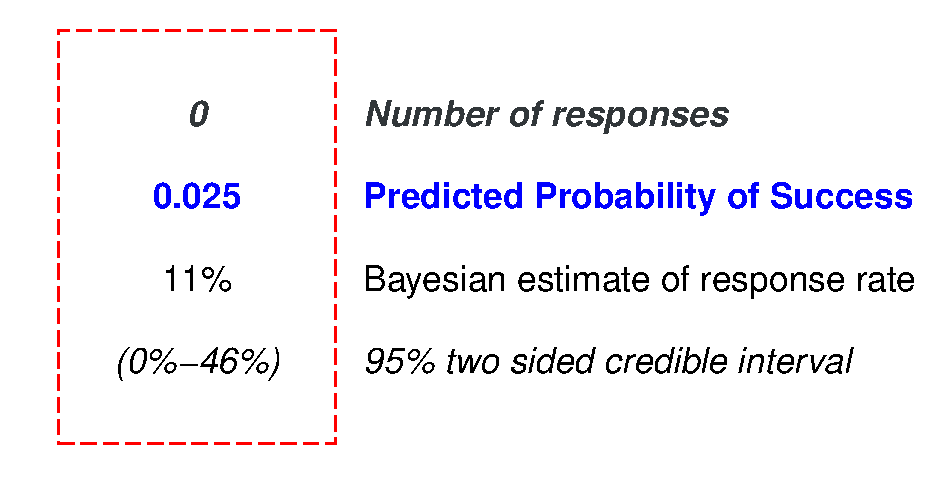
\includegraphics[width=\textwidth]{ETP-cell0Resp5Pat}
\end{figure}

The number at the top indicates the outcome for the cell, in this case the number of responses which is 0. The second row shows the PPoS in this scenario, the third row showing the Bayesian estimate of response rate and the last row shows the 95\% credible interval. For 0 responses the PPoS is 0.025 which is less than our threshold so the decision here would be to stop. This is represented by the red dashed line. From this one cell we are able to see what the decision would be at the interim analysis time point if this is the outcome that is observed. We are also able to see specifically what the PPoS and estimated response rate would be as well.  

Cells are generated for each possible outcome at each interim time point. Figure \ref{fig_etp:Cell2Resp5Pat} shows the cell for two responses in five patients. Here we can see the PPoS is 0.501 which is greater than our threshold so the decision would be made to continue recruitment. This is indicated by the green dashed line. As we put each cell together we can then clearly see the minimum number of responses required to continue recruiting.  

\begin{figure}[h!]
	\centering
	\caption{ETP cell plot for 2 responses in 5 patients.}
	\label{fig_etp:Cell2Resp5Pat}
	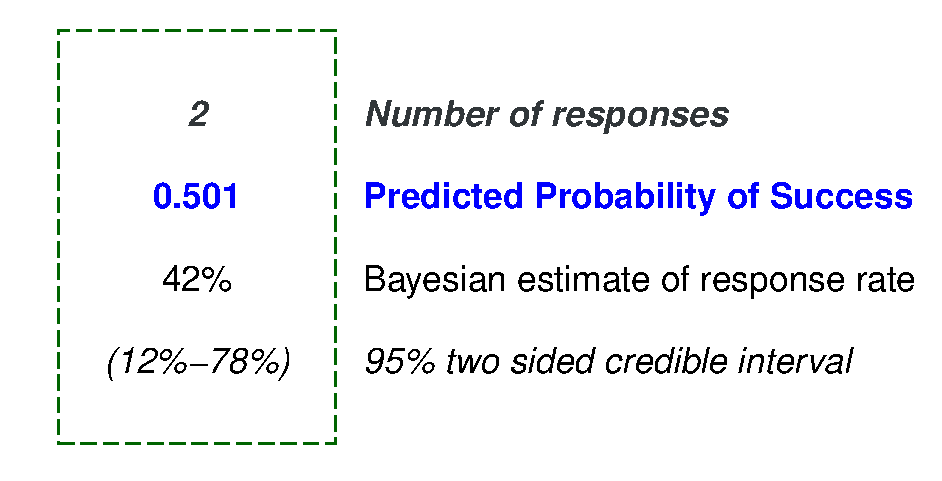
\includegraphics[width=\textwidth]{ETP-cell2Resp5Pat}
\end{figure}

This process is then repeated for each interim analysis. So, the next analysis would be at 10 patients. Here we would generate 11 cells for all the different possible outcomes (no response, one response, two responses, ..., 10 responses). The same would then be done for the analysis at 15, 20 and 25 patients. 

For the final analysis the presentation of the cells is slightly different. Here we are no longer interested in PPoS as no more patients will be recruited and rather we can just evaluate if the trial has met the decision criteria. So, in each cell rather than present PPoS the posterior probability that the response rate is greater than our target rate is presented instead. Figures \ref{fig_etp:Cell10Resp30Pat} and \ref{fig_etp:Cell14Resp30Pat} show the cells for 10 responses and 14 responses out of 30 patients respectively. In this example our $q$ is set at 0.9 so if the posterior probability is greater than that we have a GO decision. 


\begin{figure}[h!]
	\centering
	\caption{ETP cell plot for 10 responses in 30 patients.}
	\label{fig_etp:Cell10Resp30Pat}
	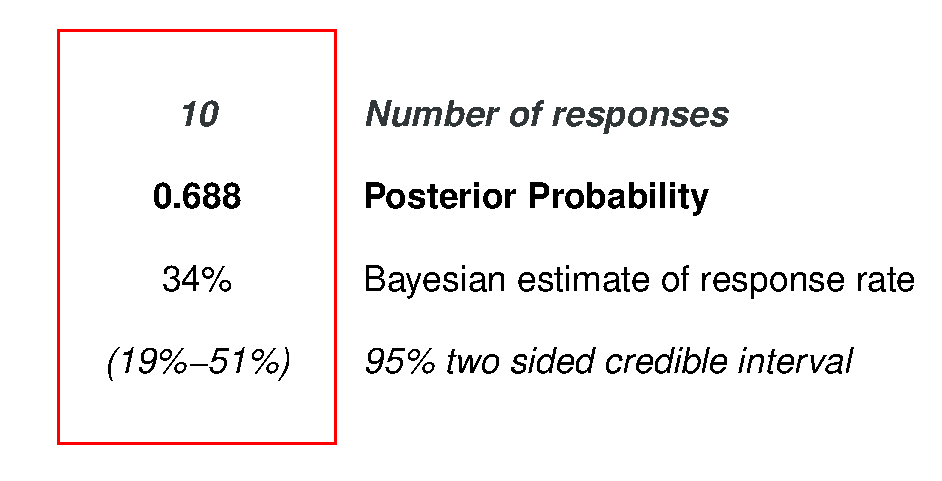
\includegraphics[width=\textwidth]{ETP-cell10Resp30Pat}
\end{figure}


\begin{figure}[h!]
	\centering
	\caption{ETP cell plot for 14 responses in 30 patients.}
	\label{fig_etp:Cell14Resp30Pat}
	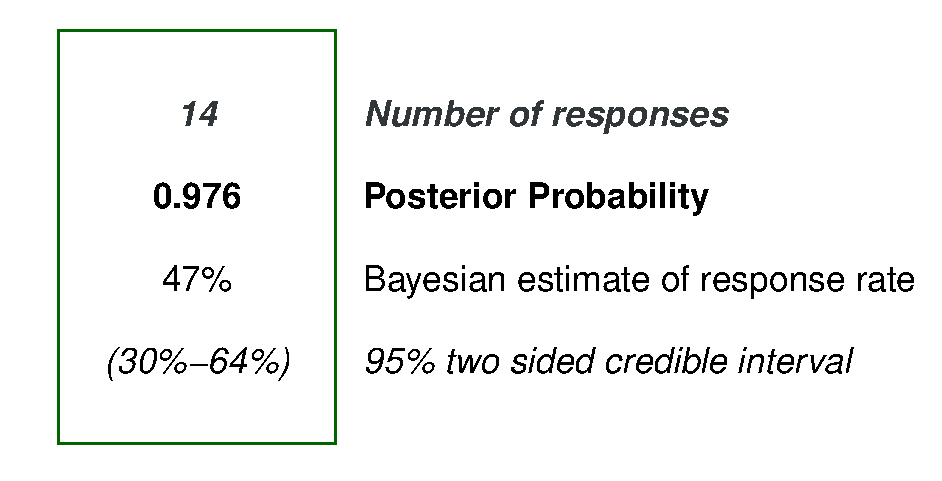
\includegraphics[width=\textwidth]{ETP-cell14Resp30Pat}
\end{figure}


The efficacy transition pathway is then constructed by grouping each cell for each interim analysis and then stacking those group of cells together. For our example trial the ETP is shown in Figure \ref{fig_etp:ConstructedETP}. Each row of cells in the ETP represents each interim analysis with the final row representing the final analysis. One adaptation made with the cells is that the confidence interval is presented across the bottom two rows in each cell just to make the figure easier to read and more scalable. 

From this figure what can clearly be seen is when we do or do not have a GO decision. At each interim of 5, 10, 15, 20, 25 patients we can see that the minimum number of responses for a GO decision is 1, 2, 4, 7 and 9 respectively. Also, for the final analysis a minimum of 13 responses is required. 

We can also evaluate some aspects of our decision rule criteria. Specifically, around $t$ our PPoS acceptable probability threshold and $q$ our threshold of sufficient evidence or the final decision. If we were to change our value of $t$ from 0.05 we can see what affect that would have on the decisions that would be made. We can identify this by looking at the PPoS in each cell for the different interims and comparing that against the new decision rule. Consider a new value of $t$ of 0.1 our interim decision rule would become PPoS $< 0.1$, so we would stop at each interim analysis if our PPoS was less than 10\%. Now the minimum number of responses for a GO decision at each interim is 1, 3, 5, 7 and 10. This has stayed the same for the interim analyses at 5 and 20 patients but has increased by 1 extra response for the other interims. We can update our ETP to reflect this change. Figure \ref{fig_etp:ConstructedETPNewPPoS} shows this new plot. The only changes here to the original ETP \ref{fig_etp:ConstructedETP} is the colour of the border around the cells for when a GO decision is made. All the calculations of PPoS, Bayesian estimates and posterior probabilities remain the same. 

Similarly, we can also check the posterior probability for the final analysis against our value of $q$. If we were to change this to 0.8 so the decision rule would now become $P(\theta  \geq 30\%) \geq 0.8$. The minimum number of responses for a GO decision at the final analysis would be 11. By looking at the final row and the cell representing the outcome for 11 patients we see here the posterior probability is 0.808. That means the probability of the response rate being greater than 30\% is 0.808 which would meet the criteria for this new decision rule. Its important to note any change made to the final analysis decision rule will have a knock on effect to decisions made at the interim analysis. This is because the final decision rule is used to calculate the PPoS. So let's say we keep the original interim analysis decision rule of stopping if PPoS $< 0.05$ but we use the new final decision rule $P(\theta  \geq 30\%) \geq 0.8$. The associated ETP for this set of rules is given in Figure 
\ref{fig_etp:ConstructedETPNewFinal}. Here the values of PPoS have changed for the interim analyses as has the minimum number of responses required for a GO decision. It is important to note that the posterior probabilities and the Bayesian estimates of response rate with it's credible interval are the same throughout these plots. They Bayesian estimates will remain unaffected by the changes in decision rules as they are calculated based on the Beta-Binomial conjugate analysis. However, the posterior probability will change if the target response rate, $c$, is different as this is just the probability that the true response rate is higher than $c$. 

Any changes made to the target response rate in the decision rule would impact the PPoS, the posterior probability and the minimum number of responses required for GO decisions at the interim and final analyses. If our target response rate was now 40\% instead of 30\% and we kept all the decision rules and parameters the same as our original example. We would have the following decision rules: stop if PPoS $< 0.05$ at each interim and GO at final if $P(\theta  \geq 40\%) \geq 0.9$. With this new target response rate at least 16 responses are required for a GO at the final analysis. The numbers at each interim also differ as well. This can be seen in Figure \ref{fig_etp:ConstructedETPNewTarget}. 

Table \ref{tab_etp:ETP_plots_summary} provides a summary of all of the ETP plots produced. This allows us to easily compare for each plot and set of decision rules the minimum number of patients required for a GO decision. This doesn't reflect all the information that is shown in each plot but just provides a brief summary. 

\begin{table}[h!]
	\centering
	\caption{Summary of the ETP figures. }
	\label{tab_etp:ETP_plots_summary}
	\resizebox{\textwidth}{!}{%
		\begin{tabular}{l|cc|cccccc}
			\hline
			\multirow{2}{*}{\textbf{Figure}} &
			\multicolumn{2}{c|}{\textbf{Decision Rules}} &
			\multicolumn{6}{l}{\textbf{Minimum Number of Responses for a GO Decision}} \\ \cline{2-9} 
			&
			\textbf{Interim} &
			\textbf{Final} &
			\textbf{N = 5} &
			\textbf{N = 10} &
			\textbf{N = 15} &
			\textbf{N = 20} &
			\textbf{N = 25} &
			\textbf{N = 30} \\ \hline
			\ref{fig_etp:ConstructedETP} & PPoS $< 0.05$ & $P(\theta  \geq 30\%) \geq 0.9$ & 1 & 2 & 4 & 7 & 9  & 13 \\
			\ref{fig_etp:ConstructedETPNewPPoS} & PPoS $< 0.10$  & $P(\theta  \geq 30\%) \geq 0.9$ & 1 & 3 & 5 & 7 & 10 & 13 \\
			\ref{fig_etp:ConstructedETPNewFinal} & PPoS $< 0.05$ & $P(\theta  \geq 30\%) \geq 0.8$ & 0 & 2 & 3 & 5 & 8  & 11 \\
			\ref{fig_etp:ConstructedETPNewTarget} & PPoS $< 0.05$ & $P(\theta  \geq 40\%) \geq 0.9$ & 1 & 3 & 6 & 9 & 12 & 16 \\
			\hline
		\end{tabular}%
	}
\end{table}

\begin{sidewaysfigure}
	\centering
	\caption{Example of a constructed ETP.}
	\label{fig_etp:ConstructedETP}
	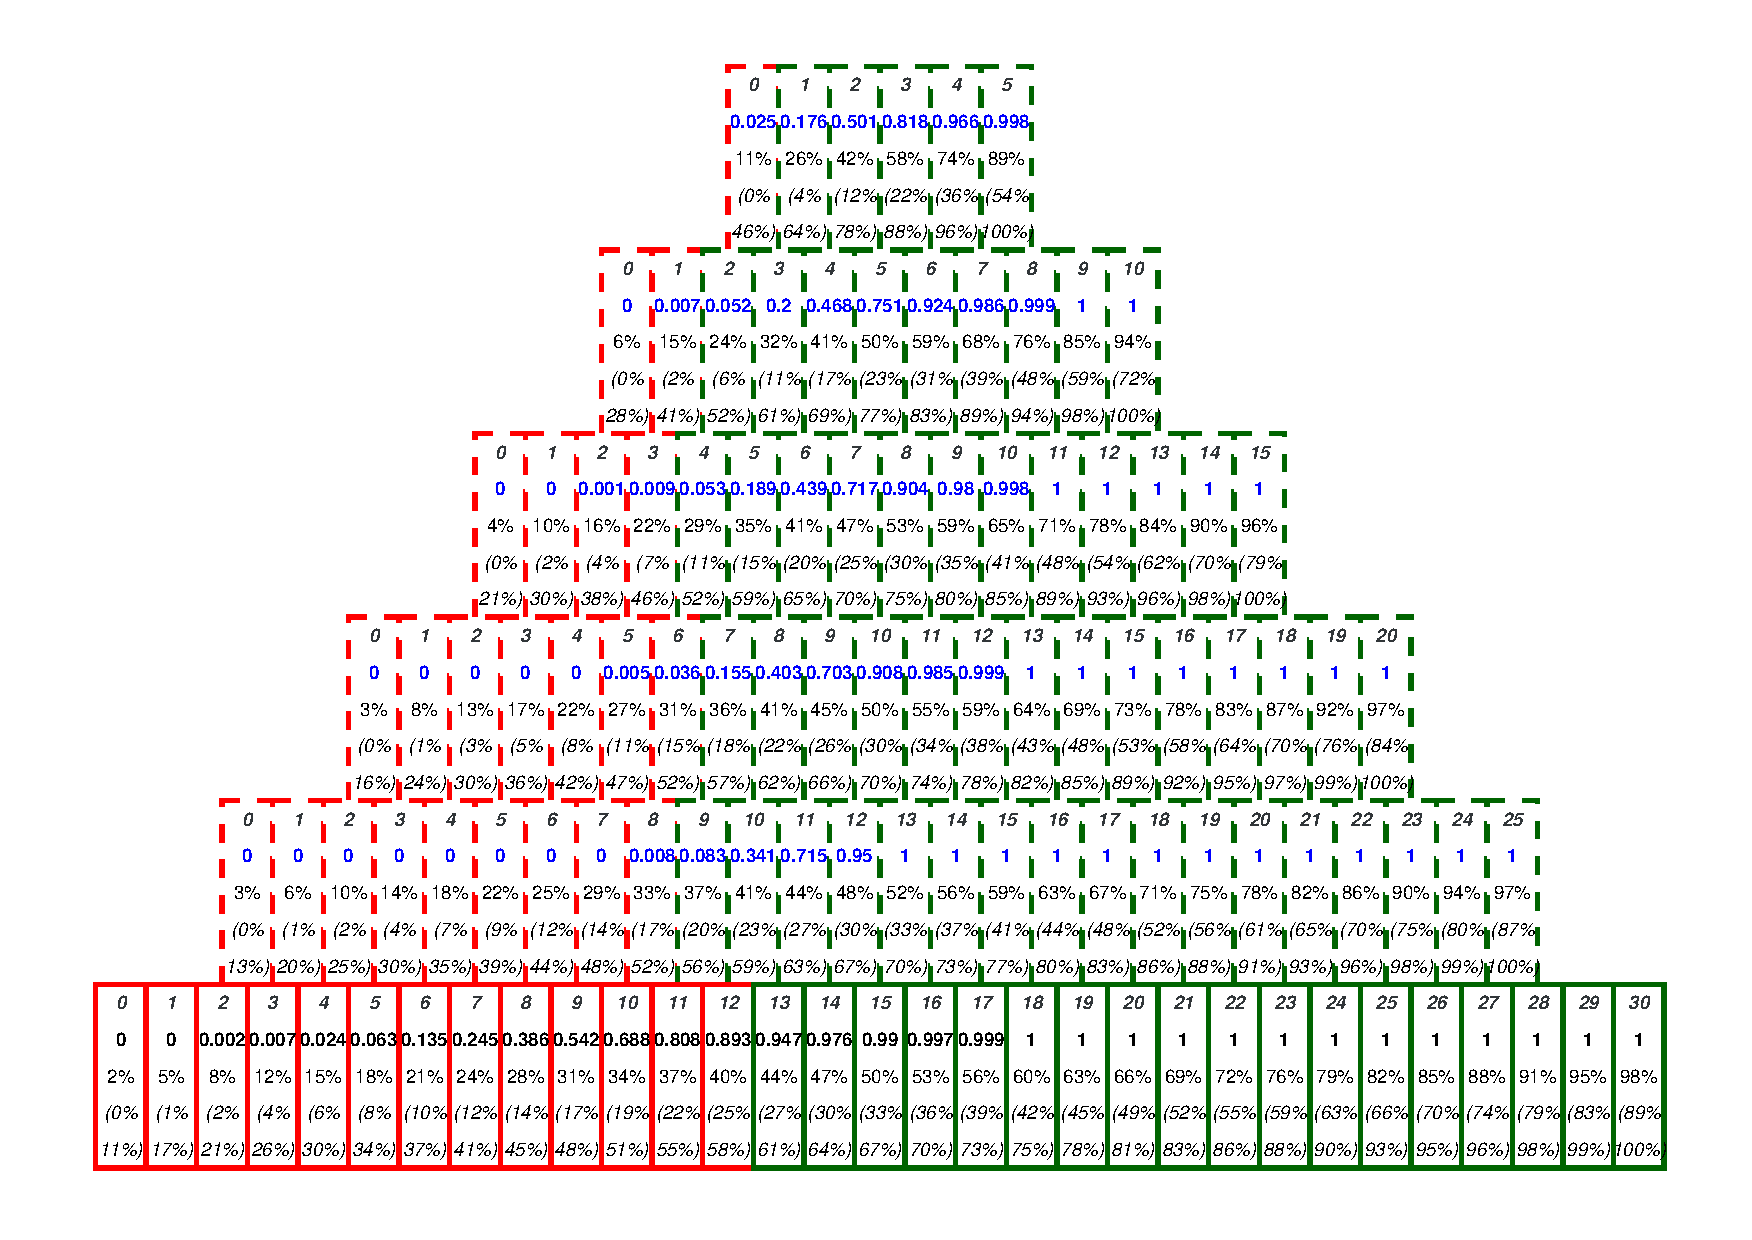
\includegraphics[width=25cm, height=15cm]{ETP-constructed}
\end{sidewaysfigure}

\begin{sidewaysfigure}
	\centering
	\caption{Example of a constructed ETP with new PPoS decision rule.}
	\label{fig_etp:ConstructedETPNewPPoS}
	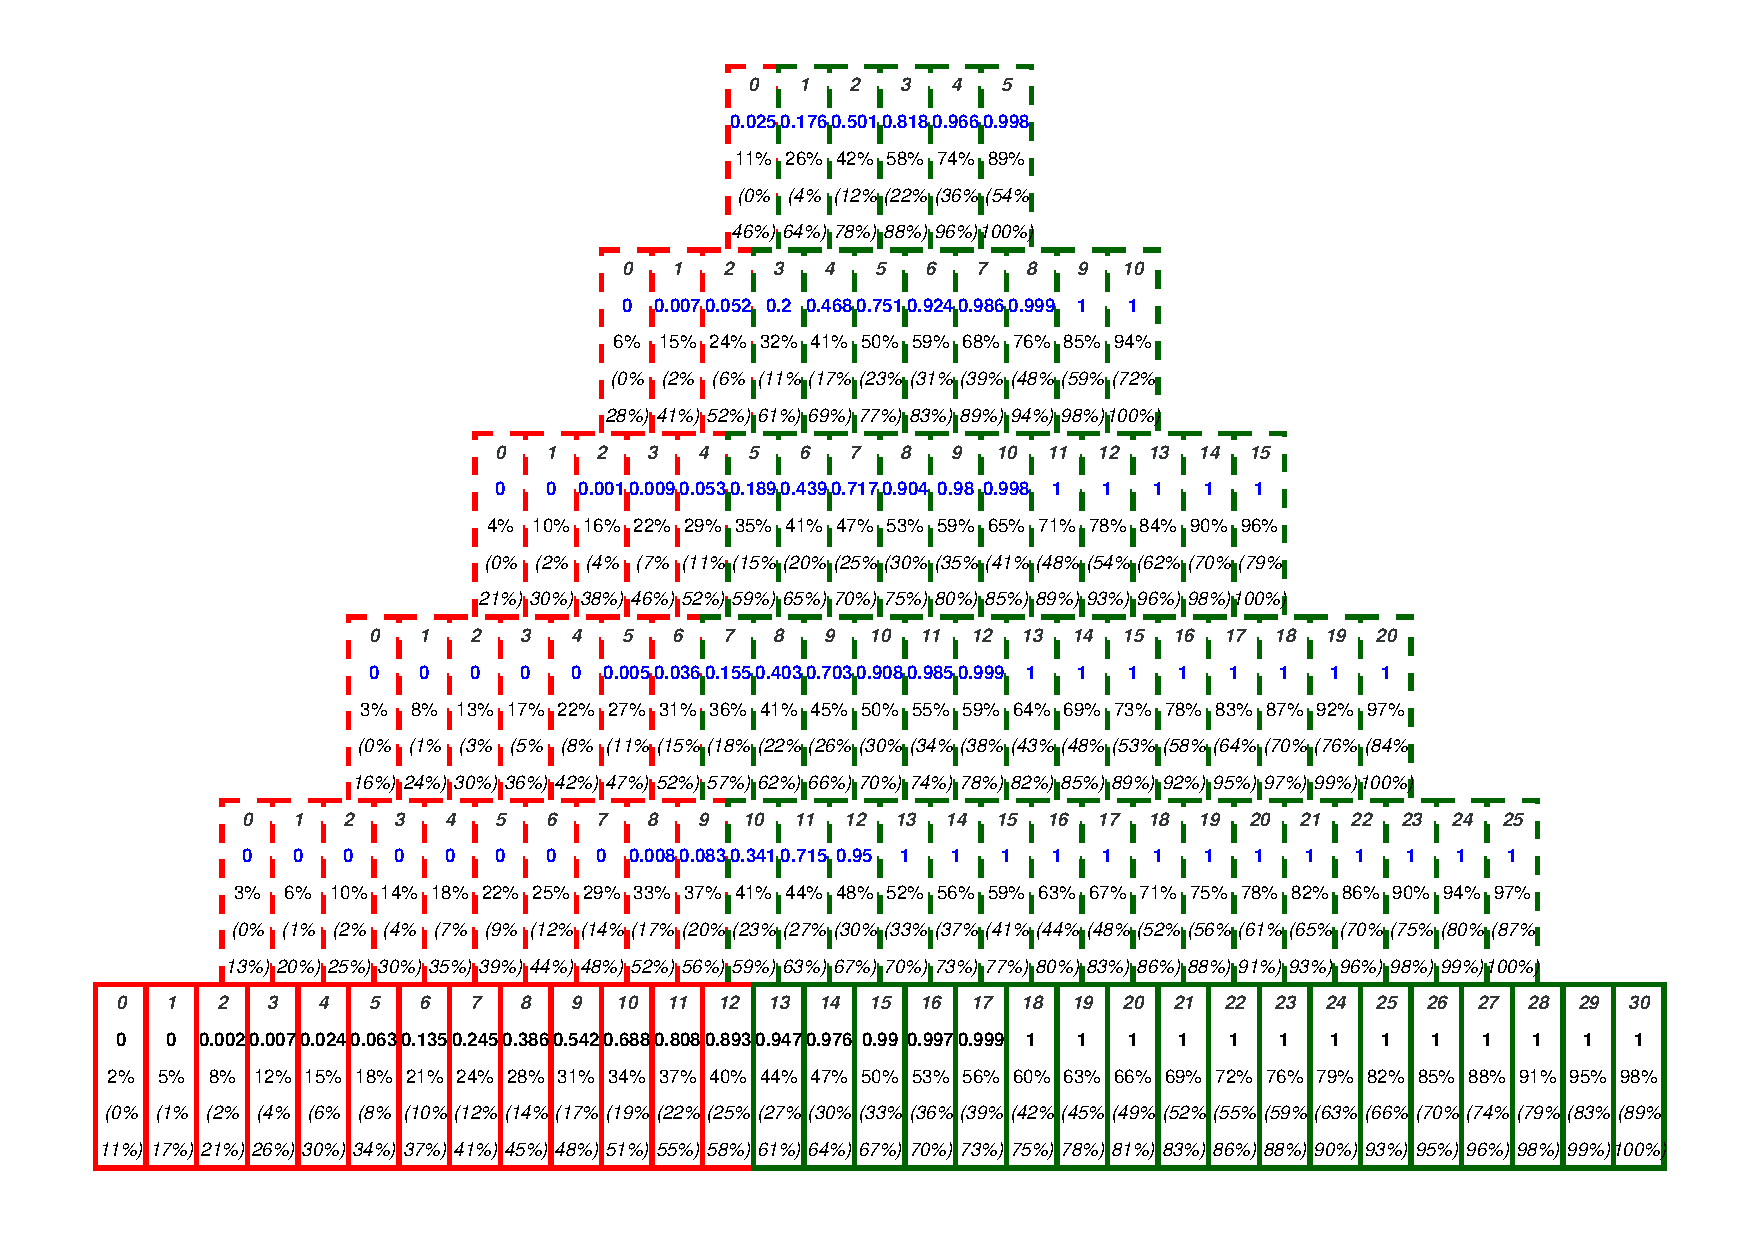
\includegraphics[width=25cm, height=15cm]{ETP-constructedNewPPoSRule}
\end{sidewaysfigure}

\begin{sidewaysfigure}
	\centering
	\caption{Example of a constructed ETP with new final decision rule.}
	\label{fig_etp:ConstructedETPNewFinal}
	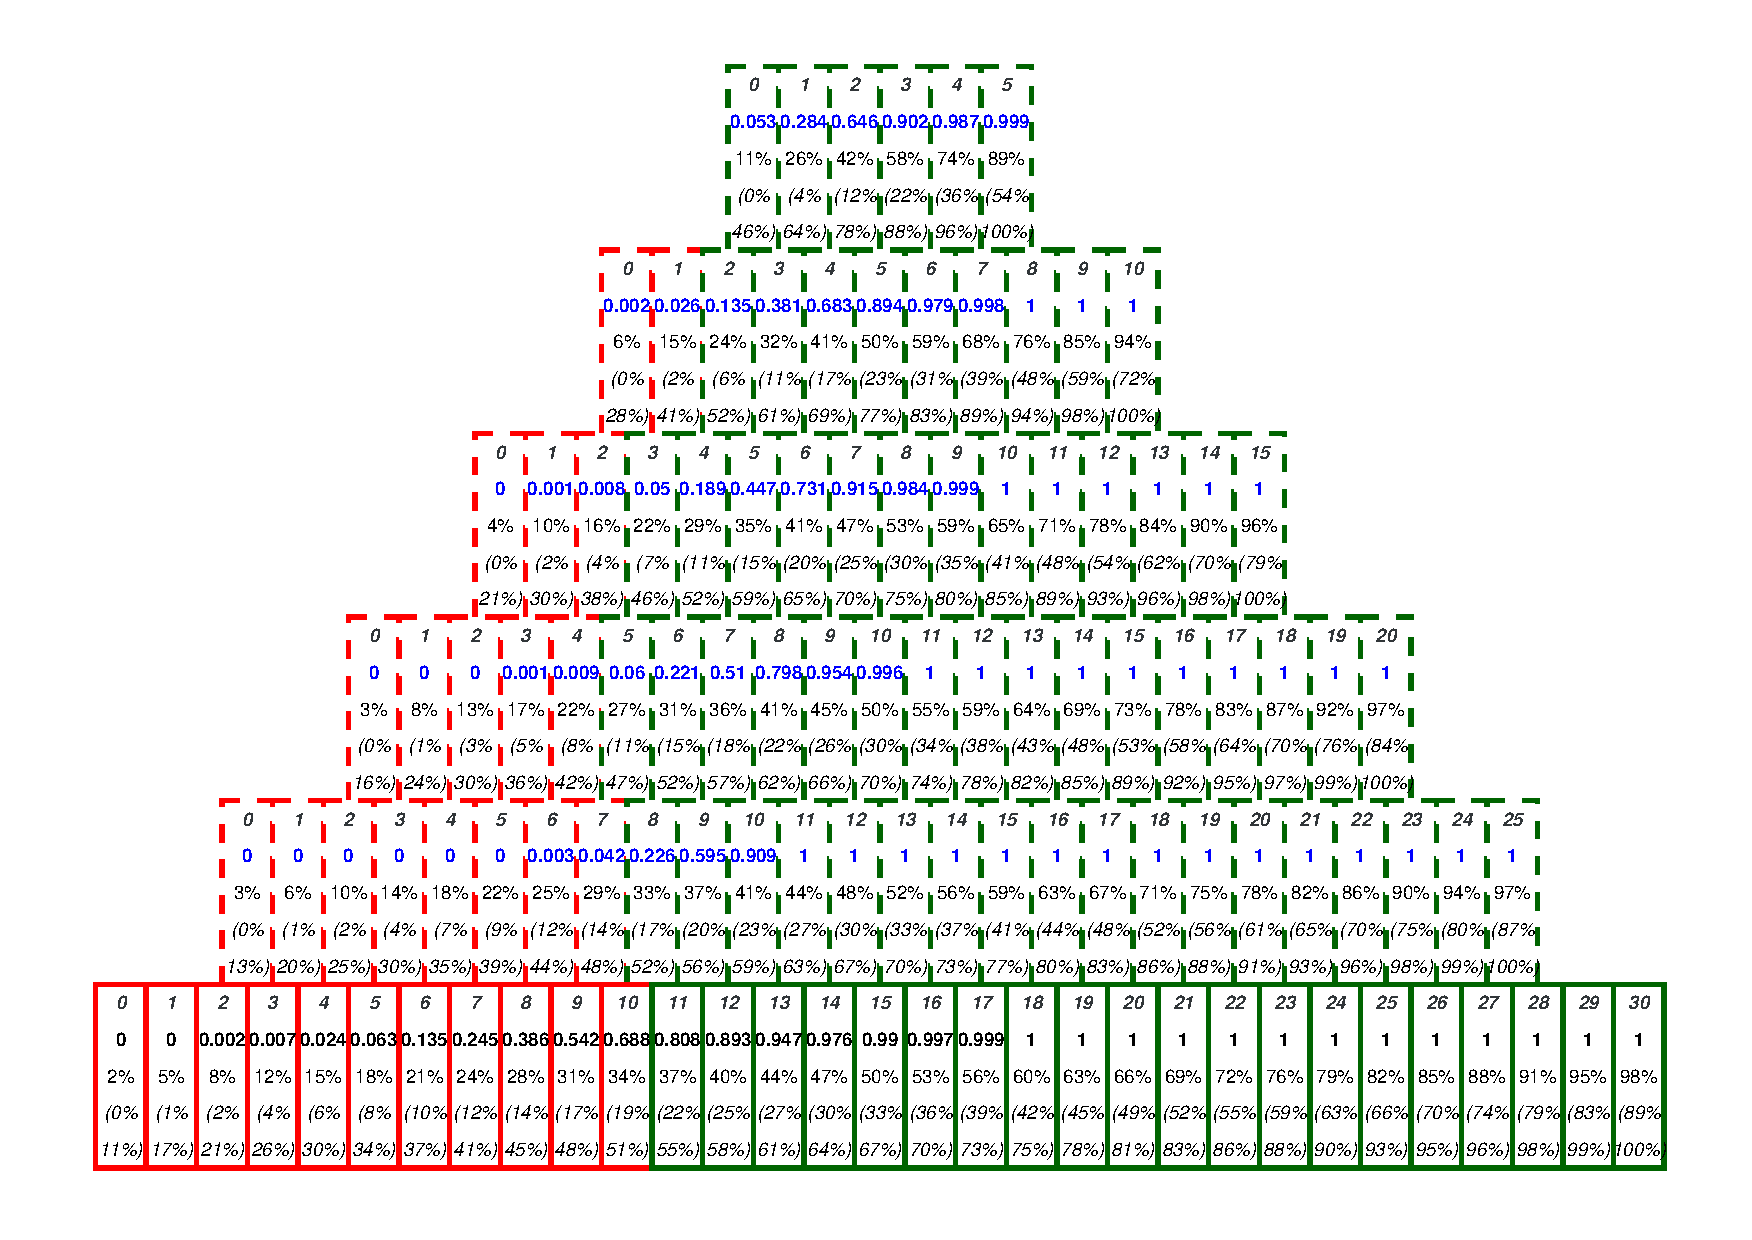
\includegraphics[width=25cm, height=15cm]{ETP-constructedNewFinalRule}
\end{sidewaysfigure}

\begin{sidewaysfigure}
	\centering
	\caption{Example of a constructed ETP with new target response rate.}
	\label{fig_etp:ConstructedETPNewTarget}
	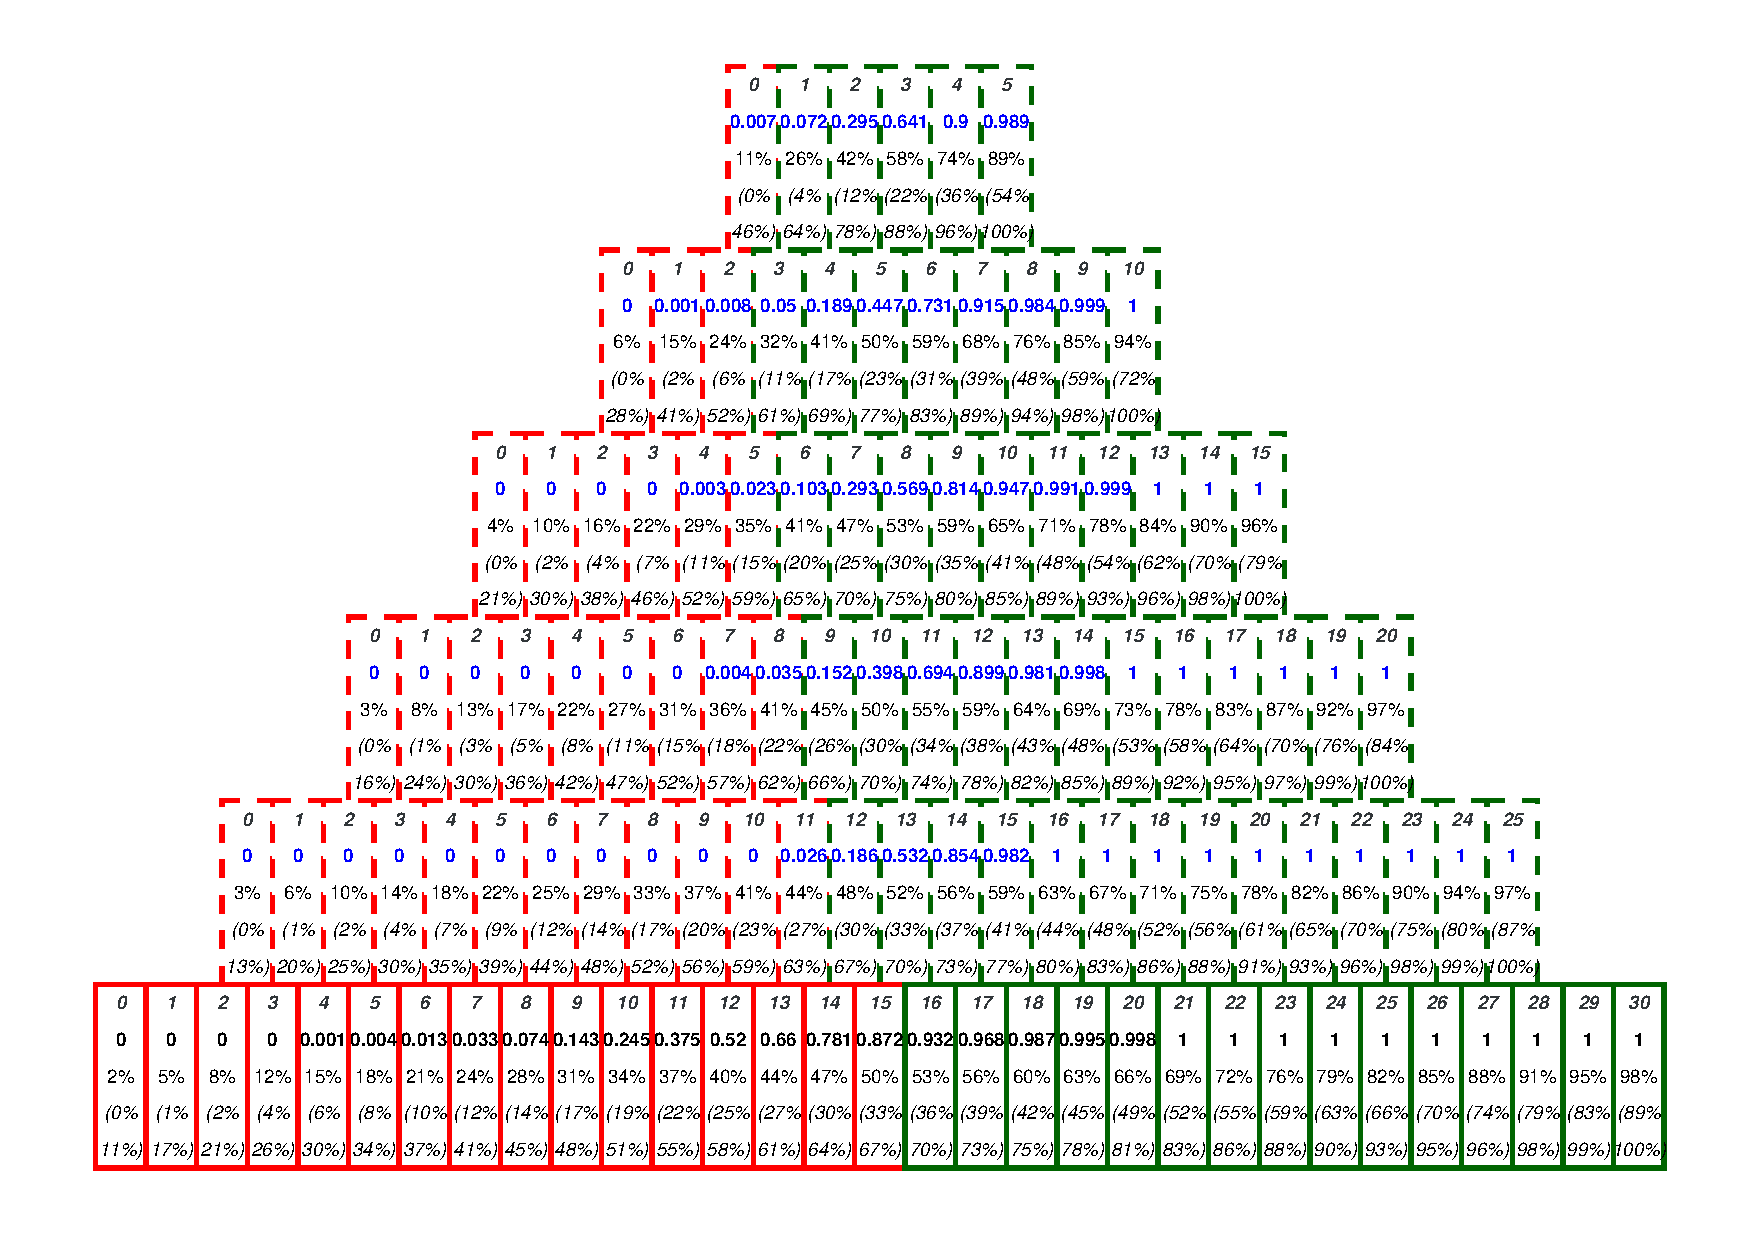
\includegraphics[width=25cm, height=15cm]{ETP-constructedNewFinalTarget}
\end{sidewaysfigure}  

\newpage

Here we have shown how ETPs are constructed and how they change and react to modifications in our decision rules. There are several other factors which can impact an ETP such as the prior used in the Beta-Binomial conjugate analysis as well as the timing of each interim analysis and the overall sample size of the trial. Changes to the prior will have an impact on all of the calculations as it is used to generate the posterior distribution on which all of the other calculations are based upon. Adding more interim analyses would add more rows to the plot and changing the sample size of the trial alters the number of cells in each row. 

Overall ETPs can be a useful tool during the design stages of a trial as we can experiment with different decision rules and see what practical affect it has on the trial in terms of the number of responses that need to be observed for a GO decision. They can be used to facilitate discussions with non statistical experts involved in the design of the trial. Much like dose transition pathways in a dose-finding trial they can also provide some transparency as to what decisions will be made and when they would be made. 

A single ETP also provides us with the ability to see how multiple different decision rules may change the outcome for a trial. If just the acceptable probability levels for the PPoS and final analysis, $t$ and $q$, are changing in the decision rule the impact of those changes should be apparent just by comparing the PPoS and posterior probability without the need of generating a whole new plot like we have in our example.

Whilst the calculations needed to produce these plots can be quite simple actually constructing the plots is not so trivial. To overcome this issue and make ETPs easily accessible and producible, we developed a web based application to generate ETPs. All the ETPs shown so far were generated using this application. 

In the next sections we detail trials that have been designed using ETPs. These served as further motivation for development of the application to produce ETPs. We then go on to detail how the app was developed and how it works.    

%----------------------------------------------------------------------------------------
%	SECTION 4
%----------------------------------------------------------------------------------------

\section{Implementation of Efficacy Transition Pathways}

With the development of any new methodology or novel tool such as ETPs there will be some barriers that will impede its use. One of those barriers will be the difficulty of implementing the methodology. If the intention of some newly developed methodology is for it be applied in a practical setting, when presented it should be accompanied by appropriate software or code such that the target audience are able to implement it with minimal effort. Otherwise the new methodology may remain purely theoretical and would rely on others to come up with a solution for its implementation. 

To overcome this barrier for ETPs we developed a R function to produce these plots given the input of key details such as the decision criteria, sample size and cohort size. We then used this function and built a web application around it. Rather than just offering code to implement ETPs a web app makes implementation even easier as it doesn't require knowledge or experience with a specific piece of stats software such as R, STATA or SAS. 

Another barrier that limits the rate at which new methodology is implemented is a lack of awareness or familiarity with the methodology. Specifically, with clinical trials that often involve a multidisciplinary team it is unrealistic to expect clinicians or trial management to be up to date with the latest statistical innovations. Even the statisticians themselves may not be familiar with the latest methodology. As a result, newer methods may be overlooked even if it would be beneficial to implement. Even if statisticians are aware of new methodology, the struggle may then become explaining the methodology to non-statisticians and convincing them it will be beneficial to use. 

Inherently ETPs as a tool were created to help better explain the analysis that is done in these phase \RN{2} trials as well as the decisions that are made. They exist more as a tool to help promote the underlying Bayesian methodology. As such there may not be that big of an issue in implementing and explaining them to non-statisticians. Rather the issue may come from not understanding the methodology behind the ETPs. 

To address this within the web application we included detailed information about ETPs as well as a breakdown of the methodology behind them. This was done through text and images in combination with custom built interactive tools that illustrates how these trials are run in a practical setting. These additional explanations and features were built in to make understanding ETPs easier, especially for those with a non stats background. These sections can also be used as a teaching tool to help educate those who are working on trials but not familiar with this methodology.  
 
Lucinda Billingham (LB) as the visionary behind ETPs had began implementing them in a number of different trial designs despite these barriers. Some of these trials were being designed as umbrella, basket or platform trials and involved multiple arms. Here analyses and decisions were being made in each arm independently so ETPs were employed to help design these trials. 

This leads to more issues where during the design stages of a trial multiple ETPs may need to be generated. If changes were made to specific decision criteria the ETP would need to be updated so you could communicate how those changes would affect the outcome of the trial. This is then further compounded with the complex trial designs where there may different criteria dependent on the arms in the trial.

Prior to the development of the app ETPs were being construct by hand which was a time consuming endeavour. We will detail three trials that were designed by the Cancer Research Clinical Trials Unit (CRCTU) at the University of Birmingham and show how ETPs have previously been implemented. 

%-----------------------------------
%	SUBSECTION 1
%-----------------------------------

\subsection{MonoGerm} 

This trial was designed by Lucinda Billingham (LB) and Laura Kirton (LK). What is presented here is the design that was used as part of a grant application which has since been accepted. The trial is currently in the process of being set-up so may be subject to some design changes before it is open. 

MonoGerm \footnote{A phase II trial of carboplatin or vinblastine monotherapy induction prior to radiotherapy for patients with intracranial germinoma} is a Phase \RN{2} trial investigating, in parallel, two single-agent chemotherapies (carboplatin or vinblastine) as monotherapy prior to standard of care radiotherapy in patients with intracranial germinoma. This trial makes use of a 'flip-flop' design for enrolment and a Bayesian approach for analysis and decision making. 

Typically intracranial germinoma is chemosensitive but it requires radiotherapy for a cure. This mainly affects a paediatric population. For patients with localised disease standard of care involves three-drug chemotherapy consisting of ifosfamide, carboplatin and etoposide followed by subsequent radiotherapy. Treatment involving multiple chemotherapies allows for reduction in radiotherapy doses and fields. However, there is still an increased burden of treatment on patients which can cause both short and long-term harm. This can lead to patients experiencing multiple toxicities such as diabetes insipidus, myelosuppression, vomiting/diarrhoea, electrolyte disturbances, renal impairment, and elevation of liver enzymes. 

The aim of the trial is to evaluate whether a single-agent chemotherapy (carboplatin or vinblastine) is non-inferior to	the standard of care multi-drug chemotherapy for inducing complete response (CR), and is associated with reduced harm and improved quality of life. The primary outcome measure will be CR based on MRI scans at 6 and 12 weeks. 

The trial will consist of two arms, one arm for carboplatin and one for vinblastine. There will be 36 patients recruited in total, 18 per arm. Patients will be enrolled in cohorts of three to each treatment-arm by the flip-flop design. This is illustrated in Figure \ref{fig_etp:MonoGermFlipFlop}. Recruitment begins in the carboplatin arm and then once three patients have been recruited recruitment is paused and then begins in the vinblastine arm. Whilst recruitment is paused in the carboplatin arm an interim analysis will be performed for that first cohort. Here primary outcome data and key safety data will be assessed. Once recruitment to the first cohort of the vinblastine arm is complete and the interim analysis for the first cohort of carboplatin patients is done recruitment can begin for the second cohort in the carboplatin arm and the interim analysis for the first cohort of vinblastine patients can be conducted. This process is then repeated for the subsequent cohorts. This design allows for continuous enrolment and monitoring of the primary outcome. 

\begin{figure}[h!]
	\centering
	\caption{Flip-flop recruitment design in the MonoGerm trial.}
	\label{fig_etp:MonoGermFlipFlop}
	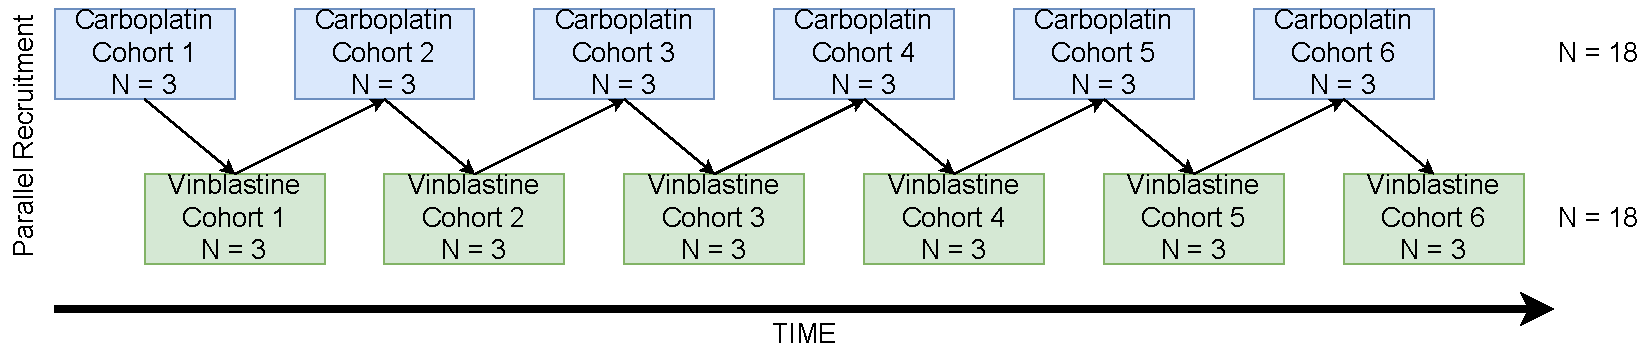
\includegraphics[width=\textwidth]{ETP-MonoGermFlipFlop}
\end{figure}

A Bayesian approach is implemented to assess the true CR rates. Specifically, the experimental monotherapies will need to demonstrate non-inferiority to the standard of care by a clinically acceptable margin. Based on previous data it was determined that the minimum CR rate with standard of care is 30\%. This value was taken as the non-inferiority margin. So, if the treatments have a CR rate $\geq30$\% they will be considered non-inferior. 

CR rates for each treatment arm will be established from the posterior probability distribution generated using a beta-binomial conjugate analysis. A minimally informative Beta(1,1) prior will be used in combination with the data observed during the trial to produce the posterior. In terms of decision making the following rule for the final analysis was specified: 

\begin{equation}
	P(CR \geq 30) \geq 0.8
\end{equation}

That is to say that if there is a high probability ($\geq 0.8$) that the true CR rate is $\geq30$\% there will be a GO decision. Which in the context of this trial means the treatment arm would be deemed non-inferior. The minimum number of observed CRs out of the 18 patients needed to warrant a GO decision is seven. If seven responses are observed the median Bayesian estimate of the CR rate would be 40\% with a 0.82 probability that the true CR rate is $\geq30$\%. 

Stopping rules have also been implemented. At each interim analysis the predicted probability of success (PPoS) will be calculated. This is the probability that a GO decision would be made at the final analysis based on current data that has been accrued. Here the stopping rule is such that if the PPoS is less than 0.01 we would recommend stopping recruitment to that arm. 

It is important to note that whilst the trial has two arms it is not designed with the intention of making comparisons between the two treatments. Rather the trial aims to find if there is enough evidence that one of these treatments provides a sufficient response rate to warrant a GO decision.  

LK produced ETPs throughout the design of this trial. Figure \ref{fig_etp:MonoGermETP} shows the ETP for the design specified here. The ETPs produced here helped determine what data we wanted to present as well as how we structure the data in each of the cells. Here each cell shows the number of responses, the PPoS or the posterior probability that the response rate is $\geq30$\%, the Bayesian estimate of CR rate and a lower one-sided 80\% credible interval.

Calculations for these plots were conducted in STATA and the ETP was produced in Microsoft PowerPoint. One benefit of this approach is that the ETP can be easily customised and labelled. However, this meant that any changes in the design that affected the decision-making resulted in the ETP having to be updated manually. As a tool the ETP is effective at illustrating a final design but without the ability to easily generate them during the design of a trial they somewhat lose their purpose. This served as further motivation to produce some code or a tool that would allow for ETPs to be automatically created. 

 
\begin{sidewaysfigure}[h!]
	\centering
	\caption{ETP for the MonoGerm trial.}
	\label{fig_etp:MonoGermETP}
	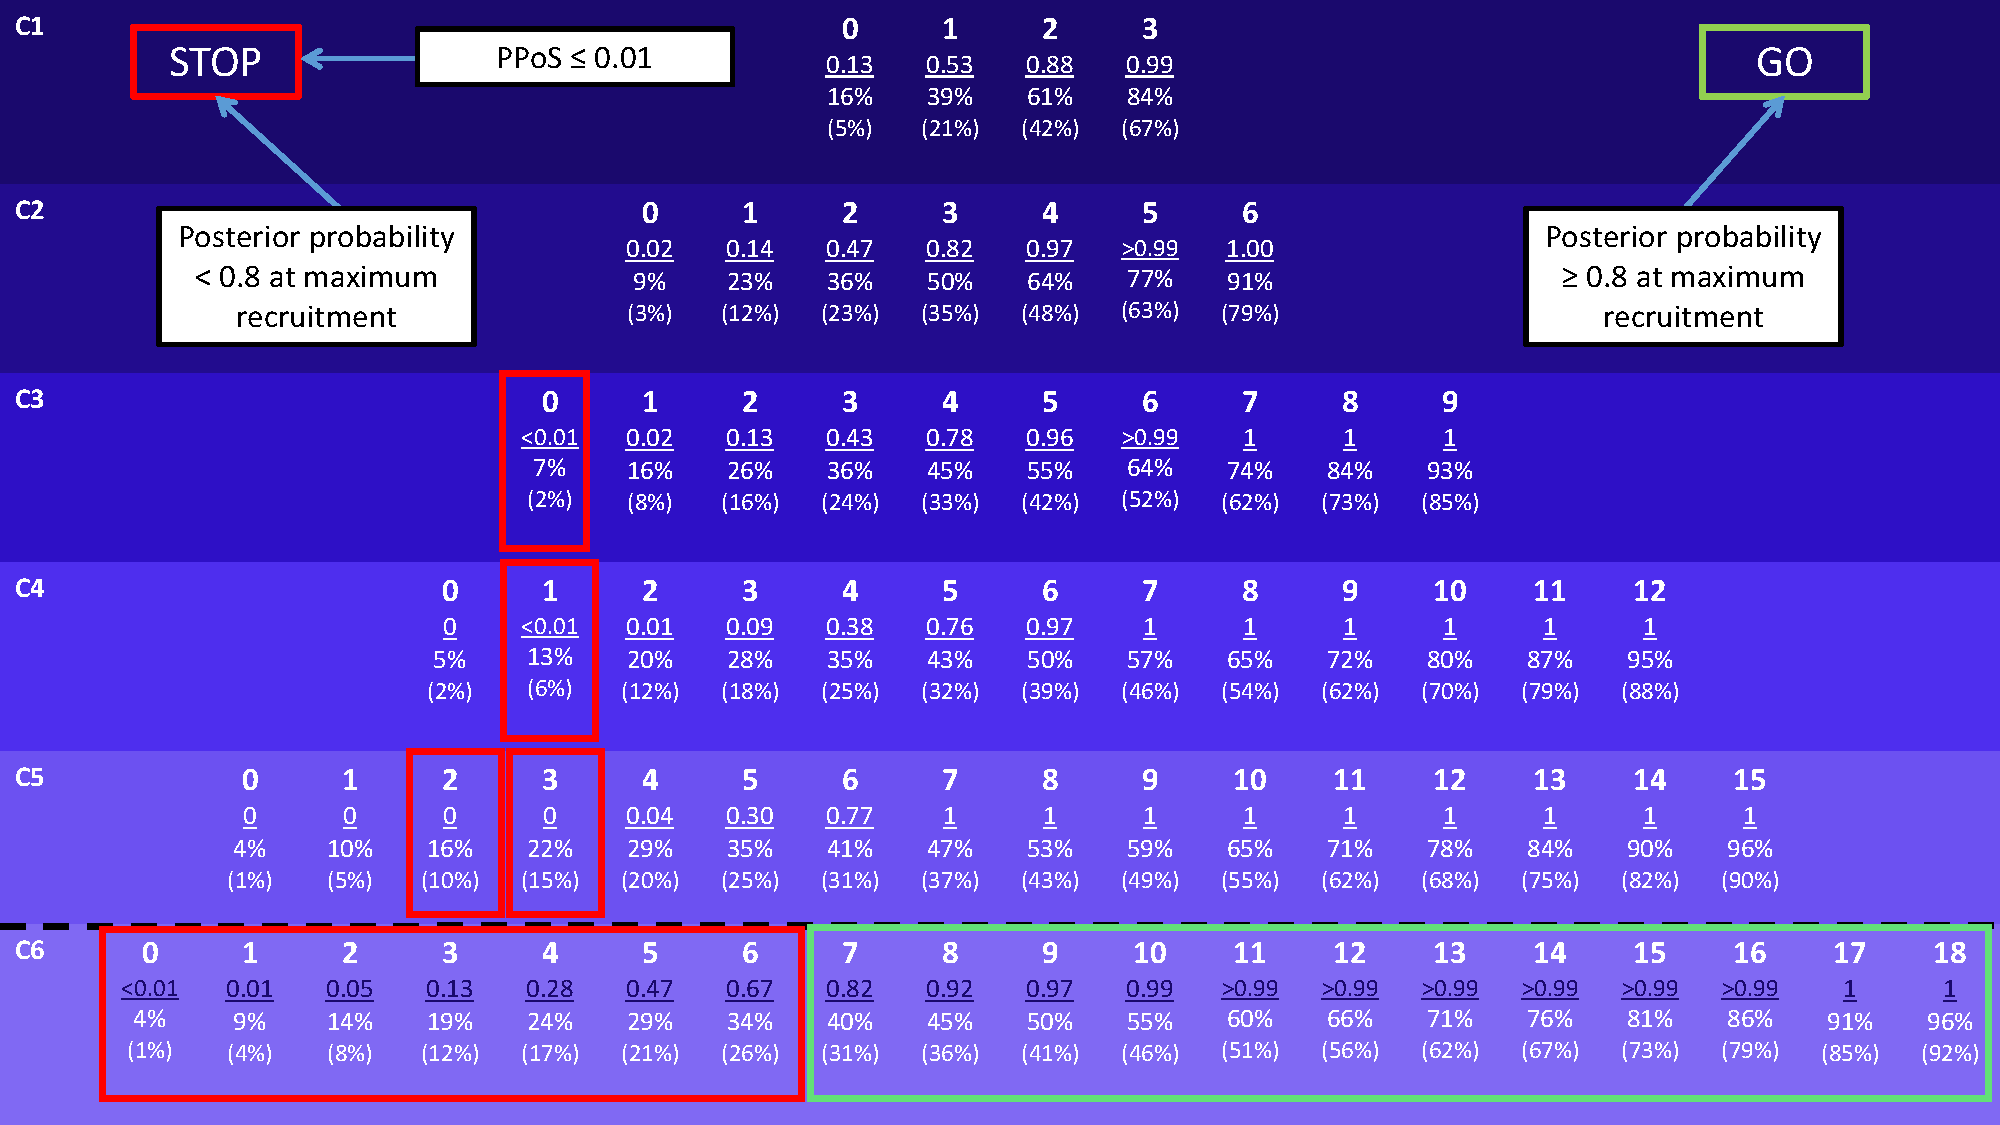
\includegraphics[width=23cm, height=15cm]{ETP-MonoGermETP}
\end{sidewaysfigure} 

 \clearpage
 
%-----------------------------------
%	SUBSECTION 2
%-----------------------------------

\subsection{Glo-BNHL}

This trial was designed by Lucinda Billingham (LB) with the assistance of Shanna Maycock (SM). During initial stages of the design Grace Holt (GH) also assisted with the implementation of ETPs. This trial is currently still in set-up so specific details of the trial may be subject to change.   

The Glo-BNHL \footnote{A Global Study of Novel Agents in Paediatric and Adolescent Relapsed and Refractory B-cell Non-Hodgkin Lymphoma} study is a platform trial that aims to investigate the safety and effectiveness of novel treatments in children, adolescents and young adults with relapsed and/or refractory B-cell non-Hodgkin Lymphoma (r/r BNHL). This trial is an international collaboration and hopes to generate substantial evidence that could change practice in this rare cancer population. 

Inclusion of novel agents into the platform will be determined by an international Trial Steering Committee (TSC). Currently the platform consists of three separate treatment arms, each focusing on a different novel agent in a distinct group of patients. Each treatment arm will be treated independently which allows for them to be analysed separately. There may also be separate eligibility criteria for each arm. Patients will be enrolled into any arm where they are eligible. The three arms that will be available at the start of the trial are as follows: 

\begin{itemize}
	\item Treatment Arm \RN{1}: Bispecific Antibody (BsAb)
	\item Treatment Arm \RN{2}: Antibody-Drug Conjugate (ADC) with standard \\ chemotherapy
	\item Treatment Arm \RN{3}: Chimeric Antigen Receptor (CAR) T-cells
\end{itemize}

This trial utilises an adaptive Bayesian design, which enables GO/No GO decisions specific to the distinct populations in each treatment arm. The Bayesian approach has many benefits here as it facilitates decision making with small sample sizes. Decisions will be made based on the estimate of the probability that a novel agent is clinically effective. The specific criteria will vary between each treatment arm. This design and approach also allows for continuous evaluation of each novel agent. Treatment arms may be removed if the treatment is shown to be ineffective based on the trial data. Additionally, treatment arms may also be added or amended in the future if recommended by the TSC. 

Treatment arm \RN{1} aims to estimate the clinical efficacy of BsAb treatment in patients with r/r BNHL in first (only one prior line of therapy) or subsequent relapse (more than one prior line of therapy). Due to this treatment arm \RN{1} is split into two groups, \RN{1}a and \RN{1}b for patients with one relapse or more than one relapse respectively. These two subsequent arms will be recruited into and analysed separately. In terms of treatment these patients will receive odronextamab given as an intravenous infusion weekly for 12 weeks, then every two weeks until nine months, and every four weeks thereafter until progression or for a maximum of two years. The outcome measure for patients in treatment arms \RN{1}a and \RN{1}b is the occurrence of an objective response (OR) i.e. complete response (CR) or partial response (PR) after 12 weeks of treatment assessed by Independent Central Review. However, for interim analyses local response assessments will be used. 

Treatment arm \RN{2} aims to estimate the clinical efficacy of ADC treatment with modified R-ICE (rituximab, ifosphamide, carboplatin, etoposide and dexamethasone) chemotherapy in patients with r/r B-NHL in first or subsequent relapse. Patients will receive loncastuximab tesirine given as a 30 minute intravenous infusion with each cycle of modified R-ICE for a maximum of three cycles. Here the outcome measure is occurrence of CR within a maximum of three cycles of treatment. 

Treatment arm \RN{3} aims to estimate the efficacy of CAR T-cell therapy in r/r B-NHL patients who have CAR T-cell product available. The specific treatments patients will receive is yet to be defined. The outcome measure is the occurrence of OR following CAR T-cell infusion. 

Each treatment arm and subsequent treatment arm (i.e. \RN{1}a and \RN{1}b) will aim to recruit 15 evaluable patients during the initial stage. Once this recruitment is complete a transition analysis is performed leading to three possible outcomes. If the analysis results in a No GO decision recruitment to that treatment arm will stop. If the analysis result is a GO decision there are two options either there is sufficient evidence to change practice so the trial will stop recruiting or this will trigger an expansion stage in which a further 15 patients will be recruited. Following the expansion stage an confirmatory analysis will be conducted on all 30 evaluable patients. 

Interim analyses will be conducted after every three patients during the initial stage and after every five patients during the expansion stage. There will also be the option to stop recruitment to a treatment arm based on the data observed in the interim analysis. Figure \ref{fig_etp:Glo-BNHLflowchart} shows a flowchart of the decision making process for each arm in the trial. 

\begin{figure}[h!]
	\centering
	\caption{Flowchart of the decision making process in Glo-BNHL.}
	\label{fig_etp:Glo-BNHLflowchart}
	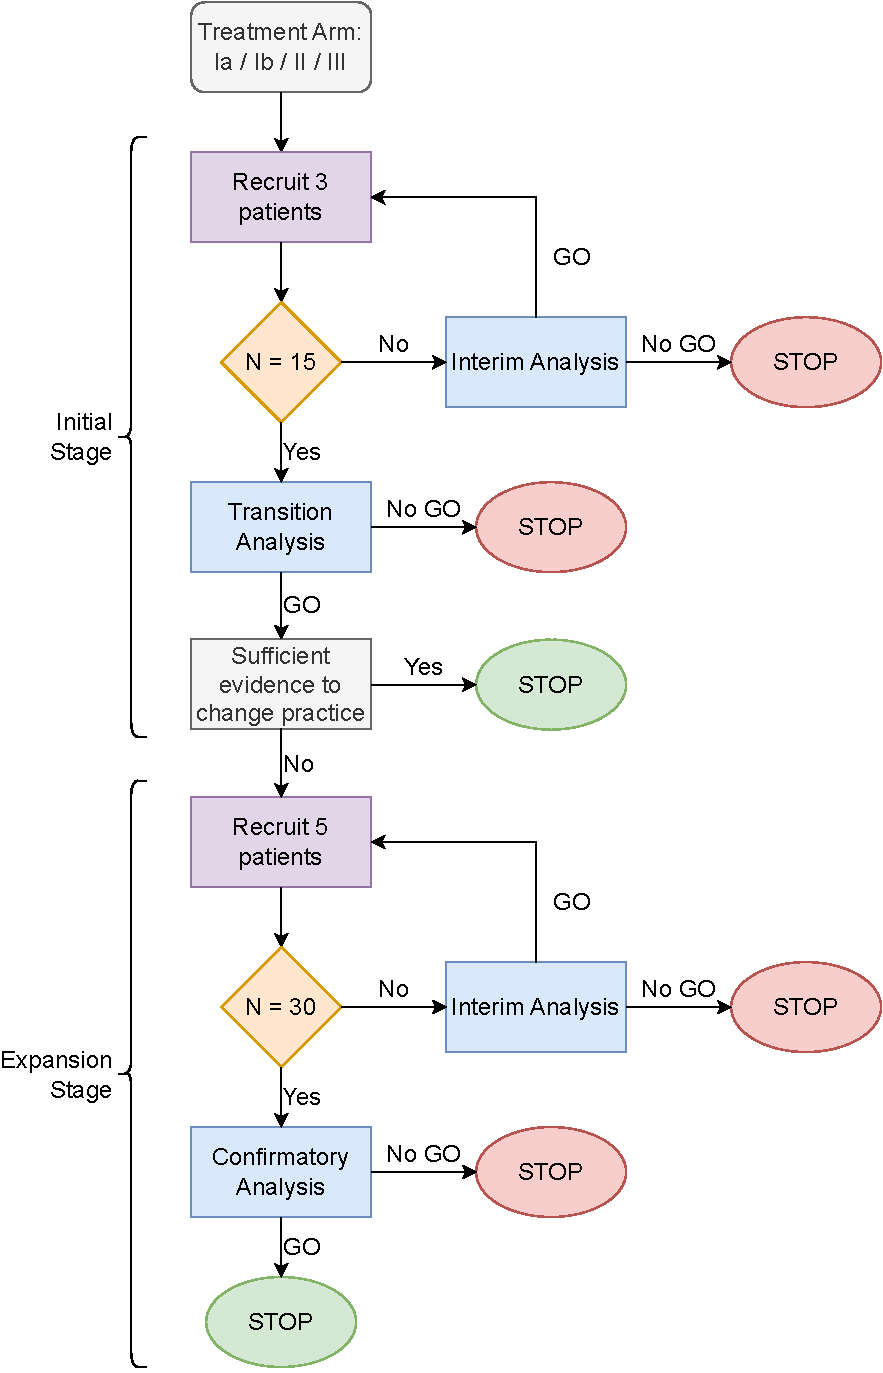
\includegraphics[width=0.9\textwidth]{ETP-GloBNHL-flowchart}
\end{figure}

A beta-binomial conjugate analysis will be conducted for each treatment arm. Observed trial data will be combined with a minimally informative Beta(1,1) prior to produce a posterior probability distribution for the treatment effect $\theta$, which represents either the OR/CR rate dependent on treatment arm. The posterior probability distribution is then used to inform decision making. GO/No Go decision criteria are specified separately for each treatment arm. 

For treatment arm \RN{1}a the decision criteria at the transition analysis is P($\theta$ > 40\%) $\geq$ 0.8. So, if the true OR rate was greater than 40\% with a probability of at least 0.8 based on the data collected in the trial there would be a GO decision. This corresponds to observing at least eight responses out of 15. For the confirmatory analysis a GO decision is made if P($\theta$ > 40\%) $\geq$ 0.95. At the final analysis we would need the probability that the true OR rate was greater than 40\% to be at least 0.95. Here a GO decision would only be made if 17 out of 30 patients had an OR. Table \ref{tab_etp:GloBNHL_decision_criteria} details the criteria for each treatment arm which can be interpreted in a similar manner. 

\begin{table}[h!]
	\centering
	\caption{Summary of decision criteria for Glo-BNHL.}
	\label{tab_etp:GloBNHL_decision_criteria}
	\resizebox{\textwidth}{!}{%
		\begin{tabular}{ccccc}
			\hline
			\multicolumn{1}{l}{\textbf{}} & \multicolumn{2}{c}{\textbf{Transition Analysis}}               & \multicolumn{2}{c}{\textbf{Confirmatory Analysis}}             \\ \cline{2-5} 
			\textbf{Treatment Arm}        & \textbf{Decision Criteria} & \textbf{Min No. Responses for GO} & \textbf{Decision Criteria} & \textbf{Min No. Responses for GO} \\ \hline
			Ia  & P($\theta$ \textgreater 40\%) $\geq$ 0.8 & 8/15 & P($\theta$ \textgreater 40\%) $\geq$ 0.95 & 17/30 \\
			Ib  & P($\theta$ \textgreater 10\%) $\geq$ 0.8 & 3/15 & P($\theta$ \textgreater 10\%) $\geq$ 0.95 & 6/30  \\
			II  & P($\theta$ \textgreater 20\%) $\geq$ 0.8 & 5/15 & P($\theta$ \textgreater 20\%) $\geq$ 0.95 & 10/30 \\
			III & P($\theta$ \textgreater 10\%) $\geq$ 0.8 & 3/15 & P($\theta$ \textgreater 10\%) $\geq$ 0.95 & 6/30  \\ \hline
		\end{tabular}%
	}
\end{table}

For the interim analyses for are separate stopping rules these are the same across the treatment arms but differ in the initial stage compared to the expansion stage. During the initial stage, the predicted probability of success at the transition analysis (PPoSt) is calculated and decisions are made based on the following criteria: 

\begin{enumerate}
	\item PPoSt < 0.01 - recommend stopping for futility
	\item 0.01 $\leq$ PPoSt < 0.05 - consider stopping for futility
	\item 0.05 $\leq$ PPoSt < 0.15 - consider whether sufficient benefit in continuing 
	\item PPoSt $\geq$ 0.15 - recommend continuing 
\end{enumerate}

So, if the probability of success at the transition analysis is less than 1\% the recommendation would be to stop recruitment to the treatment arm and if it was greater than or equal to 15\% the recommendation would be to continue recruitment. If PPoSt is between 1-5\% or 5-15\% stopping should be also be considered for either futility or if there sufficient benefit in continuing respectively.  

At the expansion stage, the predicted probability of success at the confirmatory analysis is used (PPoSc). If this is below 10\% (PPoSc < 0.1) the recommendation would be to stop recruitment to that treatment arm due to futility. It should be noted that these decision rules are only recommendations and the independent data monitoring committee (DMC) will make decisions based on not only primary outcomes but secondary outcomes, recruitment and safety data. 

For this trial ETPs were produced separately for each treatment arm and for each stage. This resulted in eight ETPs, one for the initial stage showing the outcome of the transition analysis and one for the expansion stage showing the outcome of the confirmatory analysis for each treatment arm (\RN{1}a, \RN{1}b, \RN{2}, \RN{3}). ETPs were utilised throughout the design of the trial with initial versions originally created by GH using STATA and Microsoft PowerPoint. These were then further developed by SM who performed calculations in R but still utilised PowerPoint to create the ETPs. Figure \ref{fig_etp:GloBNHL-ETP-TA1aInitial} and \ref{fig_etp:GloBNHL-ETP-TA1aExtenstion} shows the ETPs for the initial and expansion stage of treatment arm \RN{1}a respectively. These ETPs created by SM helped us determine how our function and app visually presented ETPs and we utilised a similar colour scheme. 

Similar to MonoGerm the process of creating these ETPs in PowerPoint can be time consuming. This is even more of an issue in the Glo-BNHL study due to the multiple treatment arms and stages. Additionally, this trial highlighted another issue of when you have multiple statisticians working on a trial who use different software packages. In this case it would mean work would have to be recreated in R and STATA to conduct the calculations required for ETPs. This served as further motivation for the development of an application which requires no specific stats software knowledge. As statisticians would easily be able to recreate ETPs. SM went on to further extend the function we developed to automatically generate ETPs specific to Glo-BNHL. 

\begin{sidewaysfigure}[h!]
	\centering
	\caption{ETP for the initial stage of treatment arm \RN{1}a in Glo-BNHL.}
	\label{fig_etp:GloBNHL-ETP-TA1aInitial}
	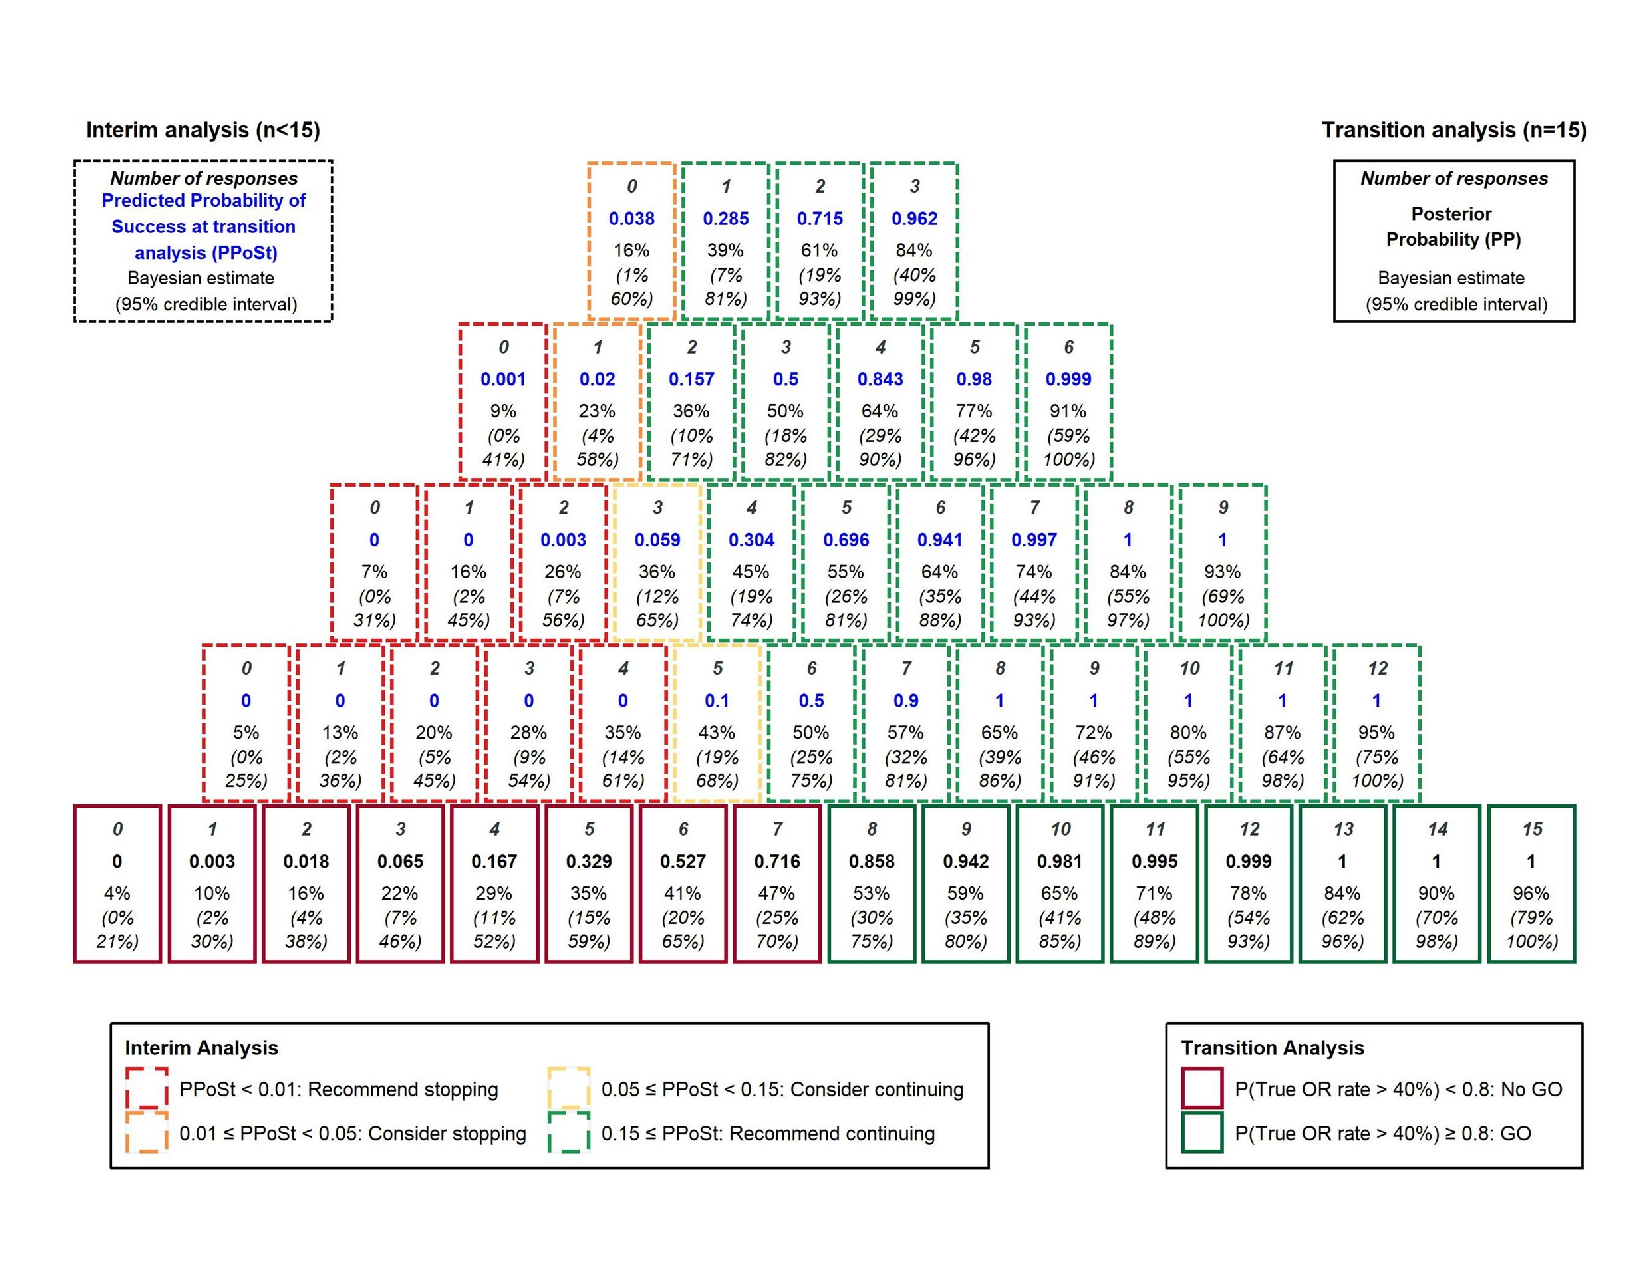
\includegraphics[width=23cm, height=15cm]{ETP-GloBNHL-ETP-TA1aInitial}
\end{sidewaysfigure} 


\begin{sidewaysfigure}[h!]
	\centering
	\caption{ETP for the expansion stage of treatment arm \RN{1}a in Glo-BNHL.}
	\label{fig_etp:GloBNHL-ETP-TA1aExtenstion}
	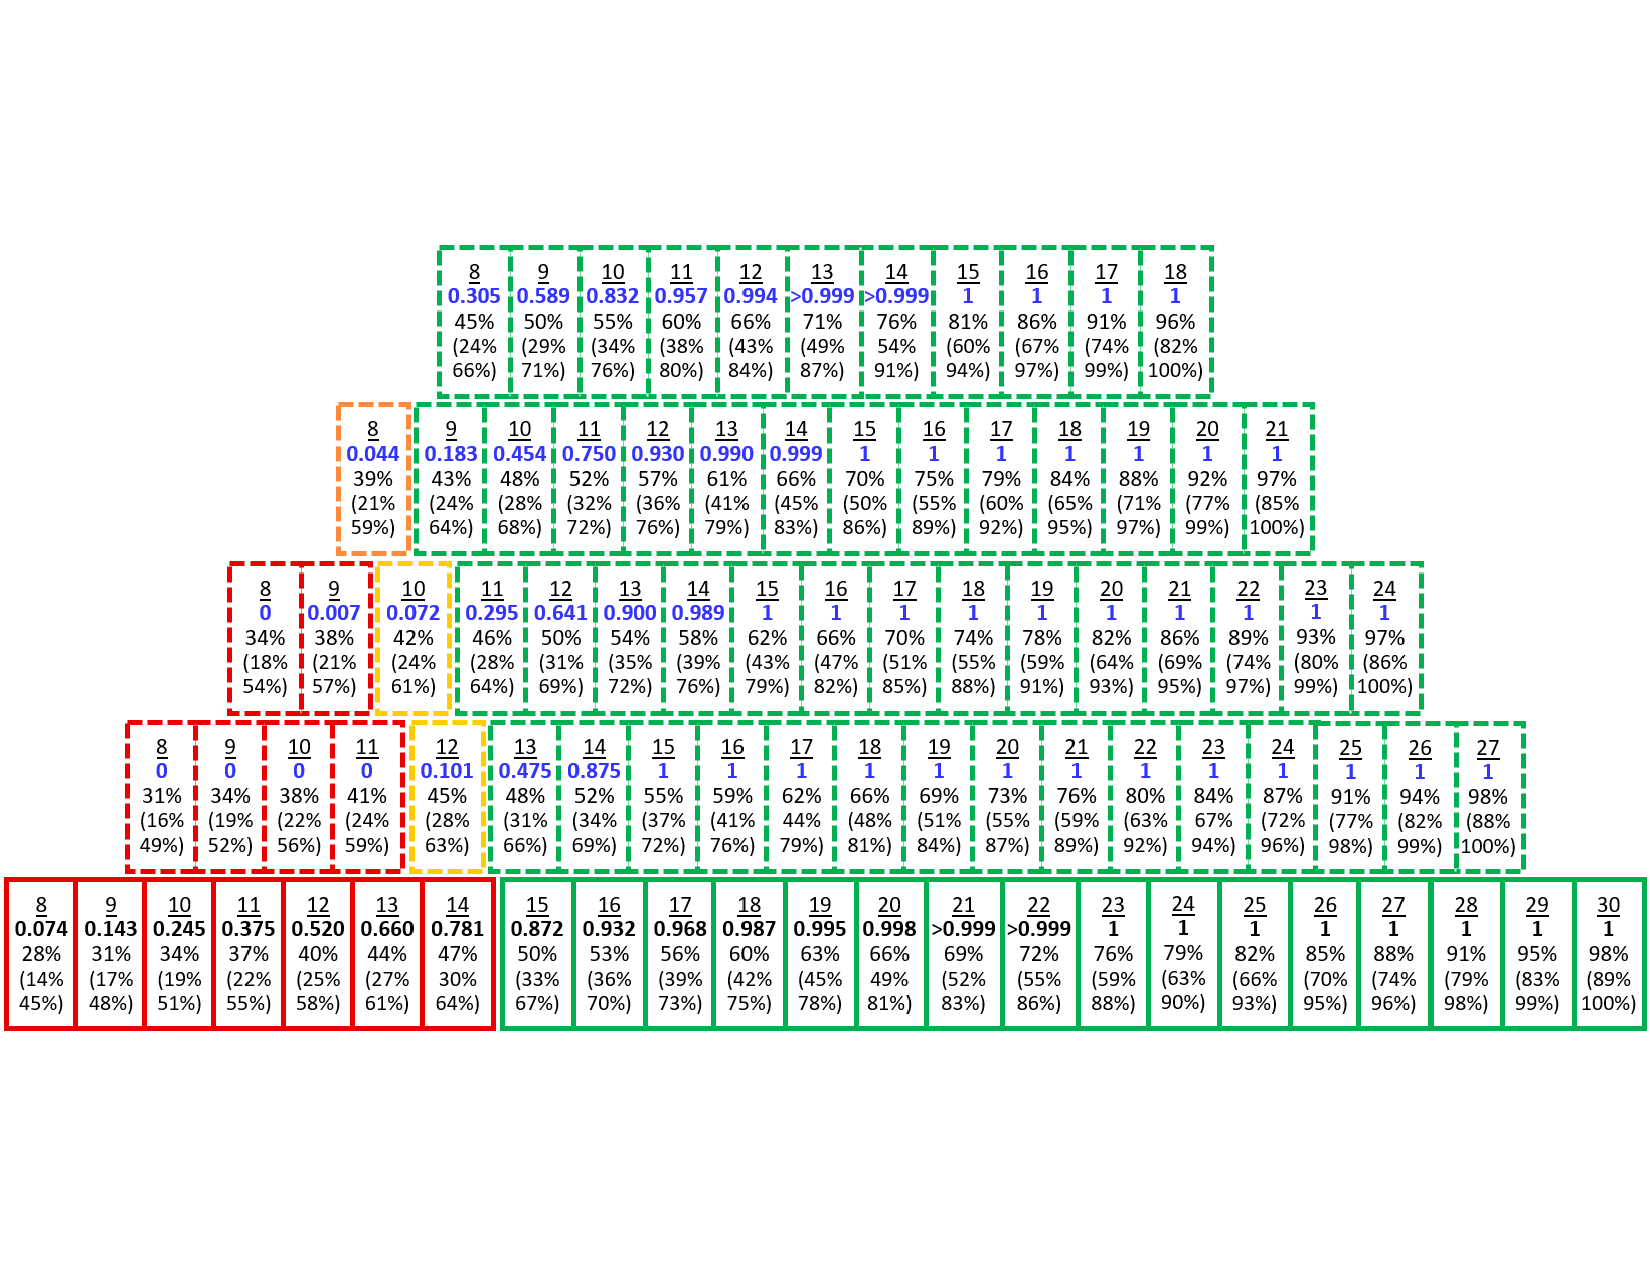
\includegraphics[width=23cm, height=15cm]{ETP-GloBNHL-ETP-TA1aExtension}
\end{sidewaysfigure} 

\clearpage


%-----------------------------------
%	SUBSECTION 3
%-----------------------------------

\subsection{DETERMINE}

DETERMINE \footnote{Determining Extended Therapeutic indications for Existing drugs in Rare Molecularly-defined Indications using a National Evaluation platform trial} is a trial that was also designed by Lucinda Billingham (LB). It is an umbrella-basket platform trial with multiple treatment arms running in parallel. The trial aims to evaluate the efficacy of targeted therapies in rare cancers with actionable genomic alterations, including common cancers with rare actionable alterations. This trial is currently open to recruitment and may be expanded in the future as more drugs are bought onto the platform.  

DETERMINE will recruit patients of all ages including, paediatric, TYA (teenage and young adult) and adults, who have rare tumours that contain an actionable genetic alteration that can be targeted therapeutically. The genetic alteration must have been identified previously from a tissue biopsy or ctDNA (circulating tumour DNA). Patients will then be stratified into molecular groups based on their tumour profile and allocated to the most suitable treatment arm by the Molecular Tumour Board (MTB). The umbrella part of the design consists of multiple non-randomised treatment arms, each evaluation a licensed targeted anti-cancer drug or drug combination in a specific molecularly-defined group of patients. Each molecularly-defined group allocated to a specific treatment arm will contain multiple baskets of different tumour types, age groups and molecular subtypes. This is visualised in Figure \ref{fig_etp:DETERMINEDesign}. 

\begin{figure}[h!]
	\centering
	\caption{Umbrella-basket platform trial design in DETERMINE.}
	\label{fig_etp:DETERMINEDesign}
	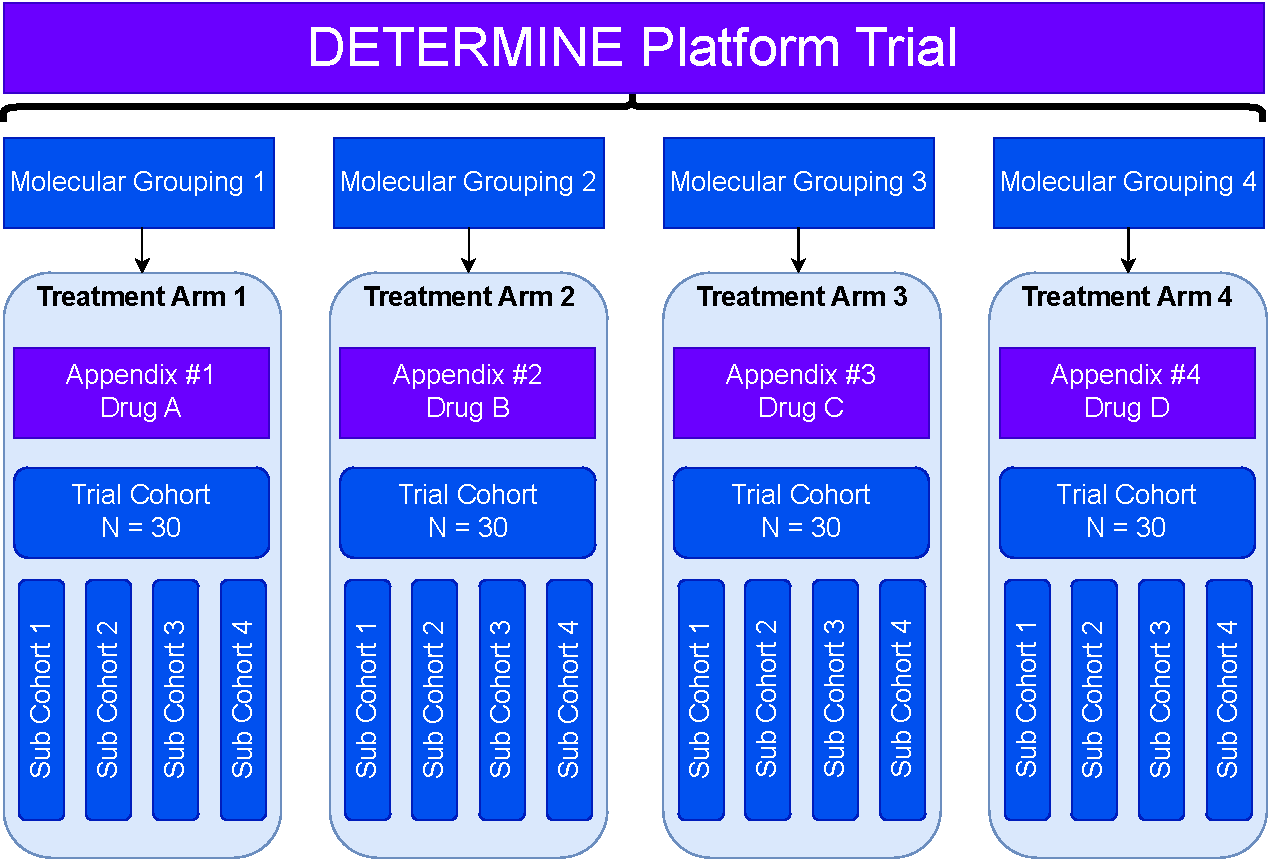
\includegraphics[width=\textwidth]{ETP-DETERMINEDesign}
\end{figure}

A main trial cohort of 30 evaluable patients will be recruited into each treatment arm. This will include patients with different tumour types, ages and molecular subtypes. If specific subgroups within this main cohort are experiencing significant benefit from treatment sub-cohorts will be formed to investigate treatment effectiveness in these subgroups. It is possible for each treatment arm to have multiple sub-cohorts and they can recruit in parallel to the main cohort. Each sub-cohort will be subject to the same statistical analysis and will also aim to recruit 30 patients. Currently there are five treatment arms, details of these are provided in Table \ref{tab_etp:DETERMINE_trtarms}. 

\begin{table}[h!]
	\fontsize{10pt}{10pt}\selectfont
	\centering
	\caption{Current treatment arms in DETERMINE}
	\label{tab_etp:DETERMINE_trtarms}
	\resizebox{\textwidth}{!}{%
		\begin{tabular}{p{0.1\textwidth} | p{0.2\textwidth} | p{0.5\textwidth} | p{0.2\textwidth}}
			Treatment Arm  & IMP(s) & Molecular Grouping & Route and Formulation \\ \hline
			1 &  Alectinib & ALK gene fusion positive solid tumours & Oral capsules \\ \hline
			2 & Atezolizumab & Solid tumours with high tumour mutational burden (TMB) or microsatellite instability-high (MSI-high) or proven constitutional mismatch repair deficiency (CMMRD) disposition & Intravenous (IV) infusion  \\ \hline
			3 & Entrectinib & NTRK or ROS1 gene fusion positive solid tumours & Oral capsules; Dosing depends on body surface area (BSA) \\ \hline
			4 & Trastuzumab in combination with pertuzumab & Solid tumours with HER2 amplification or mutations & IV infusion \\ \hline 
			5 & Vemurafenib in combination with cobimetinib & Solid tumours with BRAF V600 mutations & Oral; 960 mg tablets \\ \hline
		\end{tabular}
}
\end{table}

Co-primary outcomes of objective response (OR) and durable clinical benefit (DCB) will be used to assess efficacy of the treatment in each of the cohorts in each molecular grouping. These are both classified as binary variables. OR is defined dependent on specific disease criteria. DCB is defined as the absence of disease progression for at least 24 weeks from the start of trial treatment, this will also be measured based on disease specific criteria. Patients will receive treatment based on the license schedule for the drug in their treatment arm. Patients continue treatment till either they reach progressive disease (PD), unacceptable adverse events or withdraw from the trial. 

All outcomes in each treatment arm, cohort and sub cohort will be analysed using a Beta-Binomial conjugate analysis. Posterior probability distributions for OR and DCB will be generated using minimally informative priors, Beta(0.1,0.9) and data that is collected on the trial. However decision making will be done using the BOP-2 design \cite{zhouBOP2BayesianOptimal2017}. This design makes GO or No GO decisions by assessing posterior probabilities for a set of outcomes, which are optimised to either maximise power or minimise the number of patients. The design also allows for the control of type I and type II error rates. In DETERMINE, for each co-primary outcome, a rate of 10\% or less would represent a treatment effect that is not clinically relevant and a rate of 30\% would represent a clinically meaning full treatment effect. These can be thought of as a null and alternative hypothesis. 

Interim analyses will be conducted throughout the trial, however formal decision making will first be conducted after 10 evaluable patients have been recruited and then every 5 patients from that time-point in each cohort/sub-cohort. If probability that both the true OR and DCB rates are lower than the critical threshold of 10\% the trial would recommend stopping. The design is optimised to minimise the type II error i.e. to minimise the probability of not rejecting the null hypothesis when treatment is effective. This is done whilst controlling the type I error rate at 0.1. Under the BOP-2 design this provides the following stopping boundaries of 0/10, $\leq$1/15, $\leq$2/20, $\leq$3/25 at each of the planned analyses at 10, 15, 20 and 25 patients. For the final analysis at 30 patients there would be a GO decision if $\geq$6/30 patients had either a OR or DCB.   

The ETPs we have shown so far all have been based on a Beta-Binomial conjugate analysis with decisions made using PPoS and the posterior distribution. However, they can also be utilised here. LB created the ETP shown in Figure \ref{fig_etp:DETERMINE-ETP}. Here we can see each cell still pertains to a specific number of responses out of a certain number of patients. Bayesian estimates, credible intervals and posterior probabilities of the treatment effect being greater than our null and alternative hypothesis. The cells have then been colour coded based on the decision criteria elicited from the BOP-2 design. This trial also shows that ETPs are a flexible tool that can also be applied to trials not explicitly using a Beta-Binomial conjugate analysis for decision making. 

\begin{sidewaysfigure}[h!]
	\centering
	\caption{ETP for the DETERMINE trial.}
	\label{fig_etp:DETERMINE-ETP}
	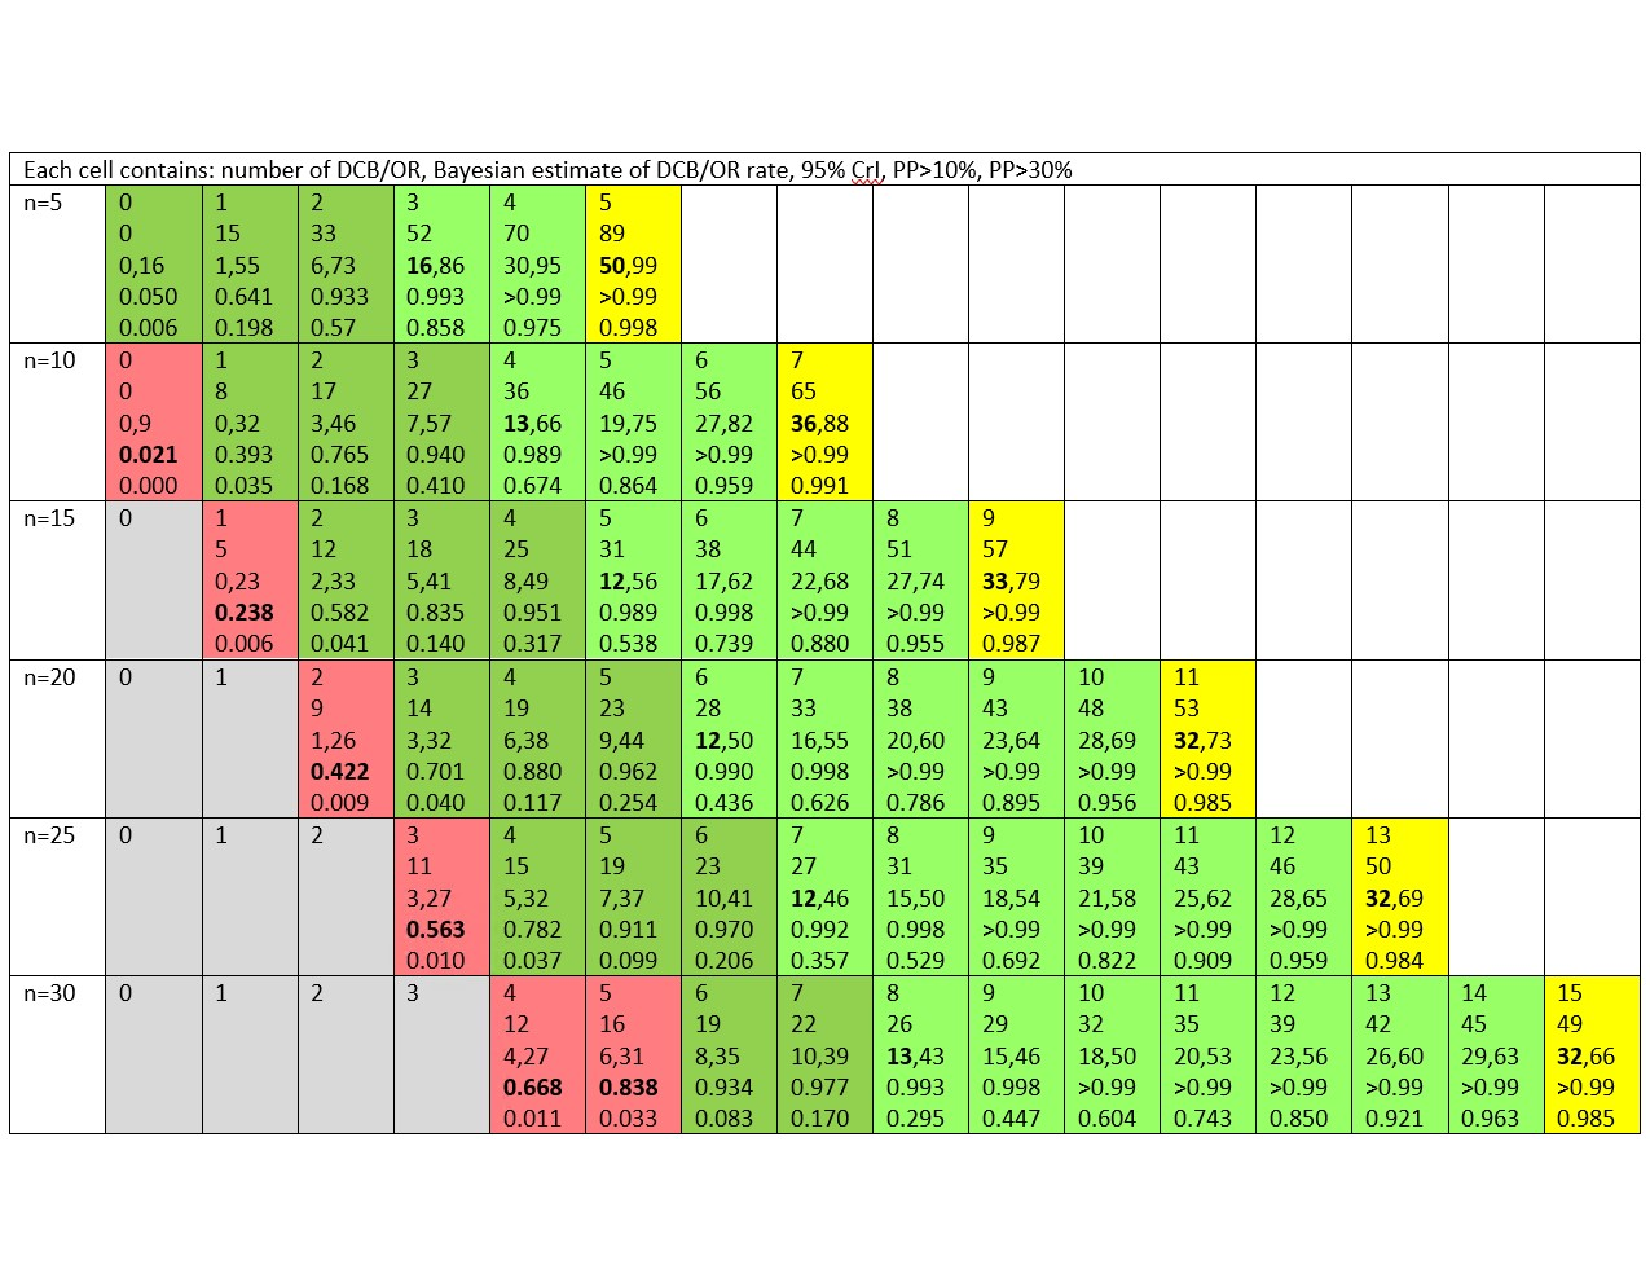
\includegraphics[width=23cm, height=15cm]{ETP-DETERMINE-ETP}
\end{sidewaysfigure} 

\clearpage
%-----------------------------------
%	SECTION 5
%-----------------------------------

\section{Development of a Web Application for Efficacy Transition Pathways}

Initially a R function was produced that was able to create ETPs. Then using R Shiny an application was built which utilised this function to produce ETPs. Whilst the R function makes implementing ETPs a lot easier the R Shiny app offers an even better solution. Firstly, it doesn't require any previous knowledge of a specific statistical package so any statistician should be able to use the application with ease. This also applies for non-statisticians and an application would make ETPs more accessible. 

R Shiny also has the ability to make graphs interactive. Whilst ETPs produce a lot of information they are static in nature. As such a change in parameters or design characteristics means that a separate ETP would need to be produced. With R shiny a interface allows for these changes to be easily made and the plots automatically be updated. Additionally, elements of interactivity can also be included in an application. In the application by clicking on a specific cell of the ETP we produce additional plots which give the user more details than they would otherwise get with just a single ETP. 

In our app we have a specific page which is labelled "plot builder" that will generate ETPs. This page is split into two sections. The section on the left can be considered as the input and the section on the right is the output. There are three tabs in the input section and each one deals with a separate set of input parameters. The prior parameters tab allows the user to specify priors that are being used in the beta-binomial conjugate analysis and also produces a plot of the corresponding beta distribution. The app can be accessed at the following link - \href{ https://amit-patel.shinyapps.io/beta-binomialapp/}{https://amit-patel.shinyapps.io/beta-binomialapp/}. 

The design parameters tab allows the user to specify the details of their trial and all the relevant information required to produce an ETP. This includes the number of cohorts and the size of each cohort, this assumes that an interim analysis will be performed once each cohort has been recruited. Details also need to be inputted regarding the decision criteria at both the interim analysis and final analysis stage. As these design parameters are inputted the output in the right hand side section named 'Decision Rules' also updates. Here the decision criteria based on the inputs are presented to the user in a mathematical format. There is also text to explain what each of the rules mean so the users can ensure they have inputted the correct details. The interpretation will also be useful for non statisticians and provide some understanding of the decision criteria and what it means.  

The final input tab is for parameters corresponding to the visualisation of the plot. These correspond to arguments within the R function which allow the user to adjust how the ETPs look. There is the ability to change the alignment of the ETP such that the cells are either centred or left aligned. There is also an option to change the size of the text in the ETP. As ETPs can become more and more complicated depending on the design of the trial the text may become over crowded so would need to be adjusted, which is what this option allows for. There is also the option to turn the legend on and off. 

In the output section the tab labelled "Efficacy Transition Pathway" contains the ETP which is generated based on all the inputs from the input section (prior, design and plot parameters). The user can clearly see what the ETP for their given design would look like. From here the user also has the ability to download the ETP in multiple formats. Any changes made to the input parameters will result in the ETP being updated. This allows for the user to easily and quickly make tweaks to the trial design and see how the decisions made would change. They can also easily save/download all versions of the ETPs they make to compare across the different designs. 

There is also an added layer of interactivity that was incorporated into the app. By clicking on an individual cell in the ETP additional information and plots will be generated. Once a cell has been clicked on a line of text will appear below the ETP which provides specific details about what each of the numbers in the cell represent. Additionally, there will also be a plot of the individual cell with added text to explain what each number in the cell represents. This will allow users to investigate and further explore individual cells. This is specifically useful in scenarios where the ETP may be large and contain many cells and some may not be clear on the ETP. Additionally, a posterior distribution plot is also generated when a user clicks on a specific cell. This will allow the user to see at the specific analysis time point what the posterior distribution of the treatment effect looks like given a specific number of responses. The plot also includes key statistics as well as the specified credible intervals. This plot is produced for all cells, even those at the interim analysis, whilst these may not be the final posterior distribution it provides a visualisation of the treatment effect at that interim analysis which can than either be compared to other time points or changes in the number of responses. 

The final tab here presents the data that is used to generate the ETP plot. Each cells data is included in a row and contains results from the PPoS and posterior probability calculations. There is also some functionality within the app that so that the data can be ordered by specific columns or searched. Additionally, this dataset can also be downloaded. This allows users to take the key data and calculations for use outside of the app. Users can also take the data and use it to create their own ETP as well. Whilst the primary objective of the app is to produce the ETP it also serves as a quick calculator for PPoS. Which is a useful feature in its own right as users could specify there design and download the data and use the PPoS values in their SAPs, protocols, grant applications etc.   

The way in which the app works is that all the parameters for the Beta-Binomial trial design and inputs for the ETP are stored. They are then fed into the R function which outputs the data table. Based on the data the function will produce the required number of cells which are then plotted on a cartesian plane. Then each of the values which make up the individual cells are plotted at fixed y coordinates. The interactive element works by registering the coordinates of where the user clicks on the ETP plot. Then it finds the coordinates of the centre of the nearest cell in a specific margin and extracts the data for that cell. That extracted data is then used to create the additional elements like the text explaining that cell, the enhanced individual cell plot and the specific posterior distribution plot. 

\subsection{Additional Features of the App}

We have shown how the app allows for easy creation of ETPs so anyone familiar with the methodology and an internet contention is just a few clicks away from being able to produce these plots. The other issue we mentioned earlier with the introduction of new methodology is lack of awareness or familiarity. In order to address this we built out additional pages in the app that act as an educational resource which provide all the prerequisite knowledge required to understand ETPs. These pages cover all the material covered in this chapter. Starting from the basics of Phase \RN{2} trials, Bayesian statistics, Beta-Binomial conjugate analyses and PPoS. The traditional way to explain new concepts would usually be through some combination of text and images and whilst we employ these to introduce more of the simpler elements of ETPs, R Shiny gives us the ability to incorporate some level of interactivity within the material. 

The navigation bar on the right hand side of the app can be used to navigate through the various pages. The "Introduction" tab contains two pages. The first is an introduction to clinical trials which contains background information on the phases of clinical trials and then goes into more detail specifically about Phase \RN{2} single-arm trials. This also serves to provide some set-up and context about when a beta-binomial conjugate analysis might be used.The second page is about Bayesian analysis, which is used to introduce Bayes' theorem and concepts like priors and likelihood. Whilst both of these pages aren't the most detailed or insightful renditions of the topics, they do provide the basic information required to use the app and create ETPs. Additionally, the content on these pages should be accessible for almost anybody regardless of their experience with clinical trials or statistics. 

The next tab in the navigation bar is labelled "Beta-Binomial Designs" which is also split into two further pages. The first page is about the basics of a Beta-Binomial conjugate analysis. Here we have a brief introduction to conjugate models and more specifically a Beta-Binomial analysis. To illustrate how it works we use some interactive elements. We start by splitting the conjugate model into its three main components the prior probability distribution, the likelihood and the posterior probability distribution.  In each of these sections we detail what these components are how they are presented mathematically and how they can be interpreted. Additionally, in each section we also include a visual representation of each component along with the ability to modify the plots. All of these plots between each of the sections interact with each other. So, for the prior section we default by showing a Beta(1,1) prior distribution. The likelihood plot shows the likelihood function which is default set to 8 responses from 15 patients. Finally, the posterior section shows the posterior probability distribution based on the prior and likelihood sections, the default here is a Beta(9, 8) based on a Beta(1,1 prior) and having 8 responses for 8 patients. Additionally, we also introduce the idea of decision criteria in the posterior probability section and on the plot we visualise the cut-off for a GO/No GO decision. The default decision criteria specified here is $P(\theta  \geq 40\%) \geq 0.8$ which based on the other defaults results in a GO decision. As well as all of these plots interacting with each other we have specified controls such that the user can change any of the parameters, data or decision rules used to generate these plots. Changes to any of these inputs results in all the corresponding plots being updated. As such the user can experiment and investigate the affect of changing any of the default specifications. For clarity, we include text statements on the interpretation that can be made from the posterior which also update automatically based on the details specified.

The second page in this tab allows the user to run a practice trial using a Beta-Binomial conjugate analysis. The previous page shows the mechanics of how the design works but that is based on knowing the final number of patients and responses.  The top left box has multiple tabs containing the instructions, decision criteria and controls that are being used. For consistency we use the same decision criteria and priors as before. We also specify a true response rate, defaulted at 50\% which is the response rate we sample patients from. Again, All of these specifications can be changed by the user. Using the "Add patient" tab the user has the option to add or remove patients from the trial. A slider between 1-10 allows the user to select how many patients they want to add and then by clicking the add patients button they can add that many patients, this can then be repeated many times. Once patients are added you will see a plot in the top right box that shows a circle for each patient, coloured green or red to indicate if they had a response or no response respectively. Patients responses are determined based on the true response rate specified earlier. The bottom left box will also produce a plot showing the posterior distribution based on the number of patients added and the number of responses. The plot has a checkbox option to display the decision criteria which will show whether or not based on the data generated and decision rule if there would be a GO decision. Then the bottom right box gives statements on the interpretation of the posterior probability distribution and decision rules in the "Analysis" tab. The "Summary Estimates" tab then provides summary estimates from the posterior with the option of including these in the plot. 

This page was developed as more of a demonstration tool which can be used to illustrate how decisions we make may end up being incorrect based on data we observe or the timing of the decision. Users have the ability to add multiple sets of patients in the form of cohorts and can see what the decision or results from the trial would be based on the data they generate. As it is based on a true response rate of 50\% they may get lucky and get enough responses from 10 patients to make a GO decision but if they were to re-run this they may get a different number of responses and hence a different result. Users then can see the affect of adding more patients or changing the decision rules or the true response rate. 

Finally, we have an "App Details" tab which contains two pages. The first one includes a list of references with external links to more material on topics covered by the app. We also, reference the R packages that were used to make the app and link to their respective CRAN pages. We also have a page for version history which details what was added, changed or updated for each version of the app. A link to the code used to create the app is also hosted on GitHub and linked for users to see.  

%----------------------------------------------------------------------------------------
%	SECTION 6
%----------------------------------------------------------------------------------------

\section{Discussion}

In this chapter we introduced the idea of Efficacy Transition Pathways. These were initially thought of as an extension to Dose Transition Pathways which are used as a visualisation tool to communicate decisions made in dose-finding trials. ETPs act in a similar manner and serve as a tool to better illustrate and communicate decisions made in single arm Phase \RN{2} trials that utilise a Beta-Binomial conjugate analysis. We detail the basics of these analyses and how posterior probability of success can be used to make decisions during trial at the interim analysis stage. Just like in dose-finding, depending on the number of outcomes we observe, i.e. number of responses, we can know ahead of time the decisions that will be made. Depending on the complexity of the design and decision rules the number of different scenarios can be difficult to comprehend. So, ETPs help visualise these scenarios. These can be beneficial for not only statisticians but other investigators involved with the design and conduct of the study. 

ETPs consist of an array of cells for each cohort in a trial, with each cell containing key information pertinent to a specific number of responses being observed in the total cohort size. Constructing ETPs requires numerous calculations to be run including determining PPoS as well as Bayesian estimates and credible intervals from the posterior distribution. These then need to be evaluated against the decision criteria to determine what the outcome of the trial would be based on the data that cell represents. This then all needs to be constructed into a larger image with multiple cells. A benefit of this approach is that the cells can be tailored to include information or other details that is felt relevant to portray. However, this whole process can be a time consuming  especially during the design stages of a trial where specifications and decision rules may constantly be changed and iterated upon.   This was further illustrated in the three examples we gave of trials where ETPs had been implemented and used. Each of these trials could be considered as using complex and innovative designs which involve multiple treatment arms with various time-points for analyses and different decision rules. Throughout the design of these trials multiple different ETPs were having to be produced in order to facilitate discussions and showcase the design of the trials. 

This is one of the issues with ETPs that motivated us to create an app and some software that would automatically produce these plots. The other motivation came from issues surrounding the introduction of new methodologies. Often times when a new methodology or tool is introduced it takes a long amount of time before it gets picked up and used by those other then the original creators of the methodology. This is often due to multiple factors such as lack of awareness about the new methodology or lack of useable code or relevant materials. From the perspective of statisticians working an applying methodology keeping up-to-date with all the latest innovations is often unfeasible. Similarly, if you do come across a new methodology, if there is access to code trying to implement the methods become a time-consuming task so we may default to standard practice or what is typically done even if it's sub-optimal. Additionally, they may also need to take on the role of explaining the new methodology to non statisticians involved in the oversight and management of the trial. This burden should fall on those developing the methodology if they want it to be used more frequently. In order to facilitate this for ETPs we created a simple R function along with a Shiny app to make ETPs more accessible and easy to explain. 

The primary feature of the app is to produce ETPs, we achieve this by having a simple to use interface which allows users to produce ETPs just by clicking a few buttons. What should be stated here is that currently there is limited flexibility with adjusting the ETPs. For example, the current app and function only allows for fixed cohort sizes and one set of decision rules. If you are working in a rare disease setting, recruitment may be fragmented so your trial may employ flexible cohort sizes as such ETPs don't allow for that but could easily be modified to have a different number of cells on each row for each cohort. Similarly, you may want to consider multiple decision rules or have more complicated rules during your interim analyses. For example, if your PPoS is between a specific range say 5\% and 15\% you may want to consider stopping but if it's definitely less than that you would want to stop and if its more you would want to continue. An example of this was given with the Glo-BNHL trial. Whilst not technically difficult to account for in our code or function these are more niche scenarios that may not be too common. As such the basic functionality of the app can still be used to investigate these things. Future versions of the code and app will be updated to allow for more of these options. Also, we have shown how ETPs can be applicable to trials that use other methodologies such as the BOP-2 design which is used in the Determine trial. So any other trial designs which offer decision making could also utilise ETPs. Work could be done on including these in our app and code to make ETPs easier to produe regardless of the underlying methodology. 

The app also serves the secondary feature of acting as an educational tool. We include materials and features which will show people  what ETPs are and how they are used as well as the very basic concepts and ideas in a beta-binomial conjugate analysis. This makes uses of R Shiny interactivity features and is a different method to introduce people to a new methodology compared to something just like a publication. The material and content included has been produced and reviewed by statisticians and whilst we feel it should be widely accessible others may disagree. As such we may pilot using the app for teaching purposes and show the contents to people of a non statistical background to see if it is appropriate. Some of the features such as the page that lets you run a practice clinical trial may be best utilised by a statistician trying to explain decision making concepts in these trials. By having control over the true objective response rate you can show how by having small numbers you are prone to making the wrong decisions or if you have strict decisions rules you may need a lot of patients to obtain GO decision. 

Away from ETPs additions could be made to the app to add additional features such as options to run simulations. The run a clinical trial page is essentially manually running one iteration of a simulation. This would also be an additional draw to use the app. Whilst simulations for a Beta-Binomial conjugate analysis aren't difficult to run by having an app or a tool that does these for you could be beneficial. R shiny could be utilised to automatically produce graphics and summary tables then the design parameters that you specify could also feed in to produce ETPs, this could all then be summarised on the web page and printed off as a pdf. This may make it so more users are inclined to use the app and thus ETPs. 

Overall, we believe ETPs to be a useful tool in detailing decision making for these types of trials. We have shown like that like with DTPs they can be used to help iterate on the design of the trial and communicate the decision making with non statisticians. To avoid many of the pitfalls of new methodology that never gets used we have created code and an app which is publicly available that will easily produce these plots and act as an educational tool. 
